\documentclass[english,11pt]{beamer}

\DeclareMathOperator{\Cov}{Cov}
\DeclareMathOperator{\Var}{Var}
\DeclareMathOperator{\E}{\mathbb{E}}
\DeclareMathOperator{\Proba}{\mathbb{P}}

\newcommand{\Covb}[2]{\ensuremath{\Cov\!\left[#1,#2\right]}}
\newcommand{\Eb}[1]{\ensuremath{\E\!\left[#1\right]}}
\newcommand{\Pb}[1]{\ensuremath{\Proba\!\left[#1\right]}}
\newcommand{\Varb}[1]{\ensuremath{\Var\!\left[#1\right]}}

% norm
\newcommand{\norm}[1]{\| #1 \|}

\newcommand{\indep}{\rotatebox[origin=c]{90}{$\models$}}





\usepackage{mathptmx,amsmath,amssymb,graphicx,bibentry,bbm,babel,ragged2e}

\makeatletter

\newcommand{\noun}[1]{\textsc{#1}}
\newcommand{\jitem}[1]{\item \begin{justify} #1 \end{justify} \vfill{}}
\newcommand{\sframe}[2]{\frame{\frametitle{#1} #2}}

\newenvironment{centercolumns}{\begin{columns}[c]}{\end{columns}}
%\newenvironment{jitem}{\begin{justify}\begin{itemize}}{\end{itemize}\end{justify}}

\usetheme{Warsaw}
\setbeamertemplate{footline}[text line]{}
\setbeamercolor{structure}{fg=purple!50!blue, bg=purple!50!blue}

\setbeamersize{text margin left=15pt,text margin right=15pt}

\setbeamercovered{transparent}


\@ifundefined{showcaptionsetup}{}{%
 \PassOptionsToPackage{caption=false}{subfig}}
\usepackage{subfig}

\usepackage[utf8]{inputenc}
\usepackage[T1]{fontenc}

\usepackage{multirow}


\makeatother

\begin{document}





\title{A systematic comparison of interaction models for systems of cities}

\author{J.~Raimbault$^{1,2,\ast}$\\
\texttt{juste.raimbault@polytechnique.edu}
}


\institute{$^{1}$Complex Systems Institute, Paris, UPS CNRS 3611 ISC-PIF\\
$^{2}$UMR CNRS 8504 G{\'e}ographie-cit{\'e}s
}


\date{CCS 2018\\\smallskip
\textit{Session Infrastructure, Planning and Environment}\\\smallskip
Thessaloniki\\\smallskip
September 24th 2018
}

\frame{\maketitle}




\sframe{The long time memory of urban systems}{

% Working in geography has this advantage that we always situate in an interesting object of study, and reflexivity is therin inevitable.
% I have taken the habit to open my talks with some local context, and this one will not fail this rule, especially because of the beauty and hostory of Thessaloniki.
% Urban systems are fascinating as they are truly multi-scalar, both in time and space. In particular, they have a very long temporcal memory, partly because of the pphysical artifats : here the Rotunda Galerius which was later a chruch and a Mosque, or the white tower constructed by the ottoman empire ; but also because of non-ergodic dynamics.
% In this geo-hostorical context, understanding urban growth is a real challenge : to what extent the different relation of a given city influence its current growth and its future trajectory ?

\centering

	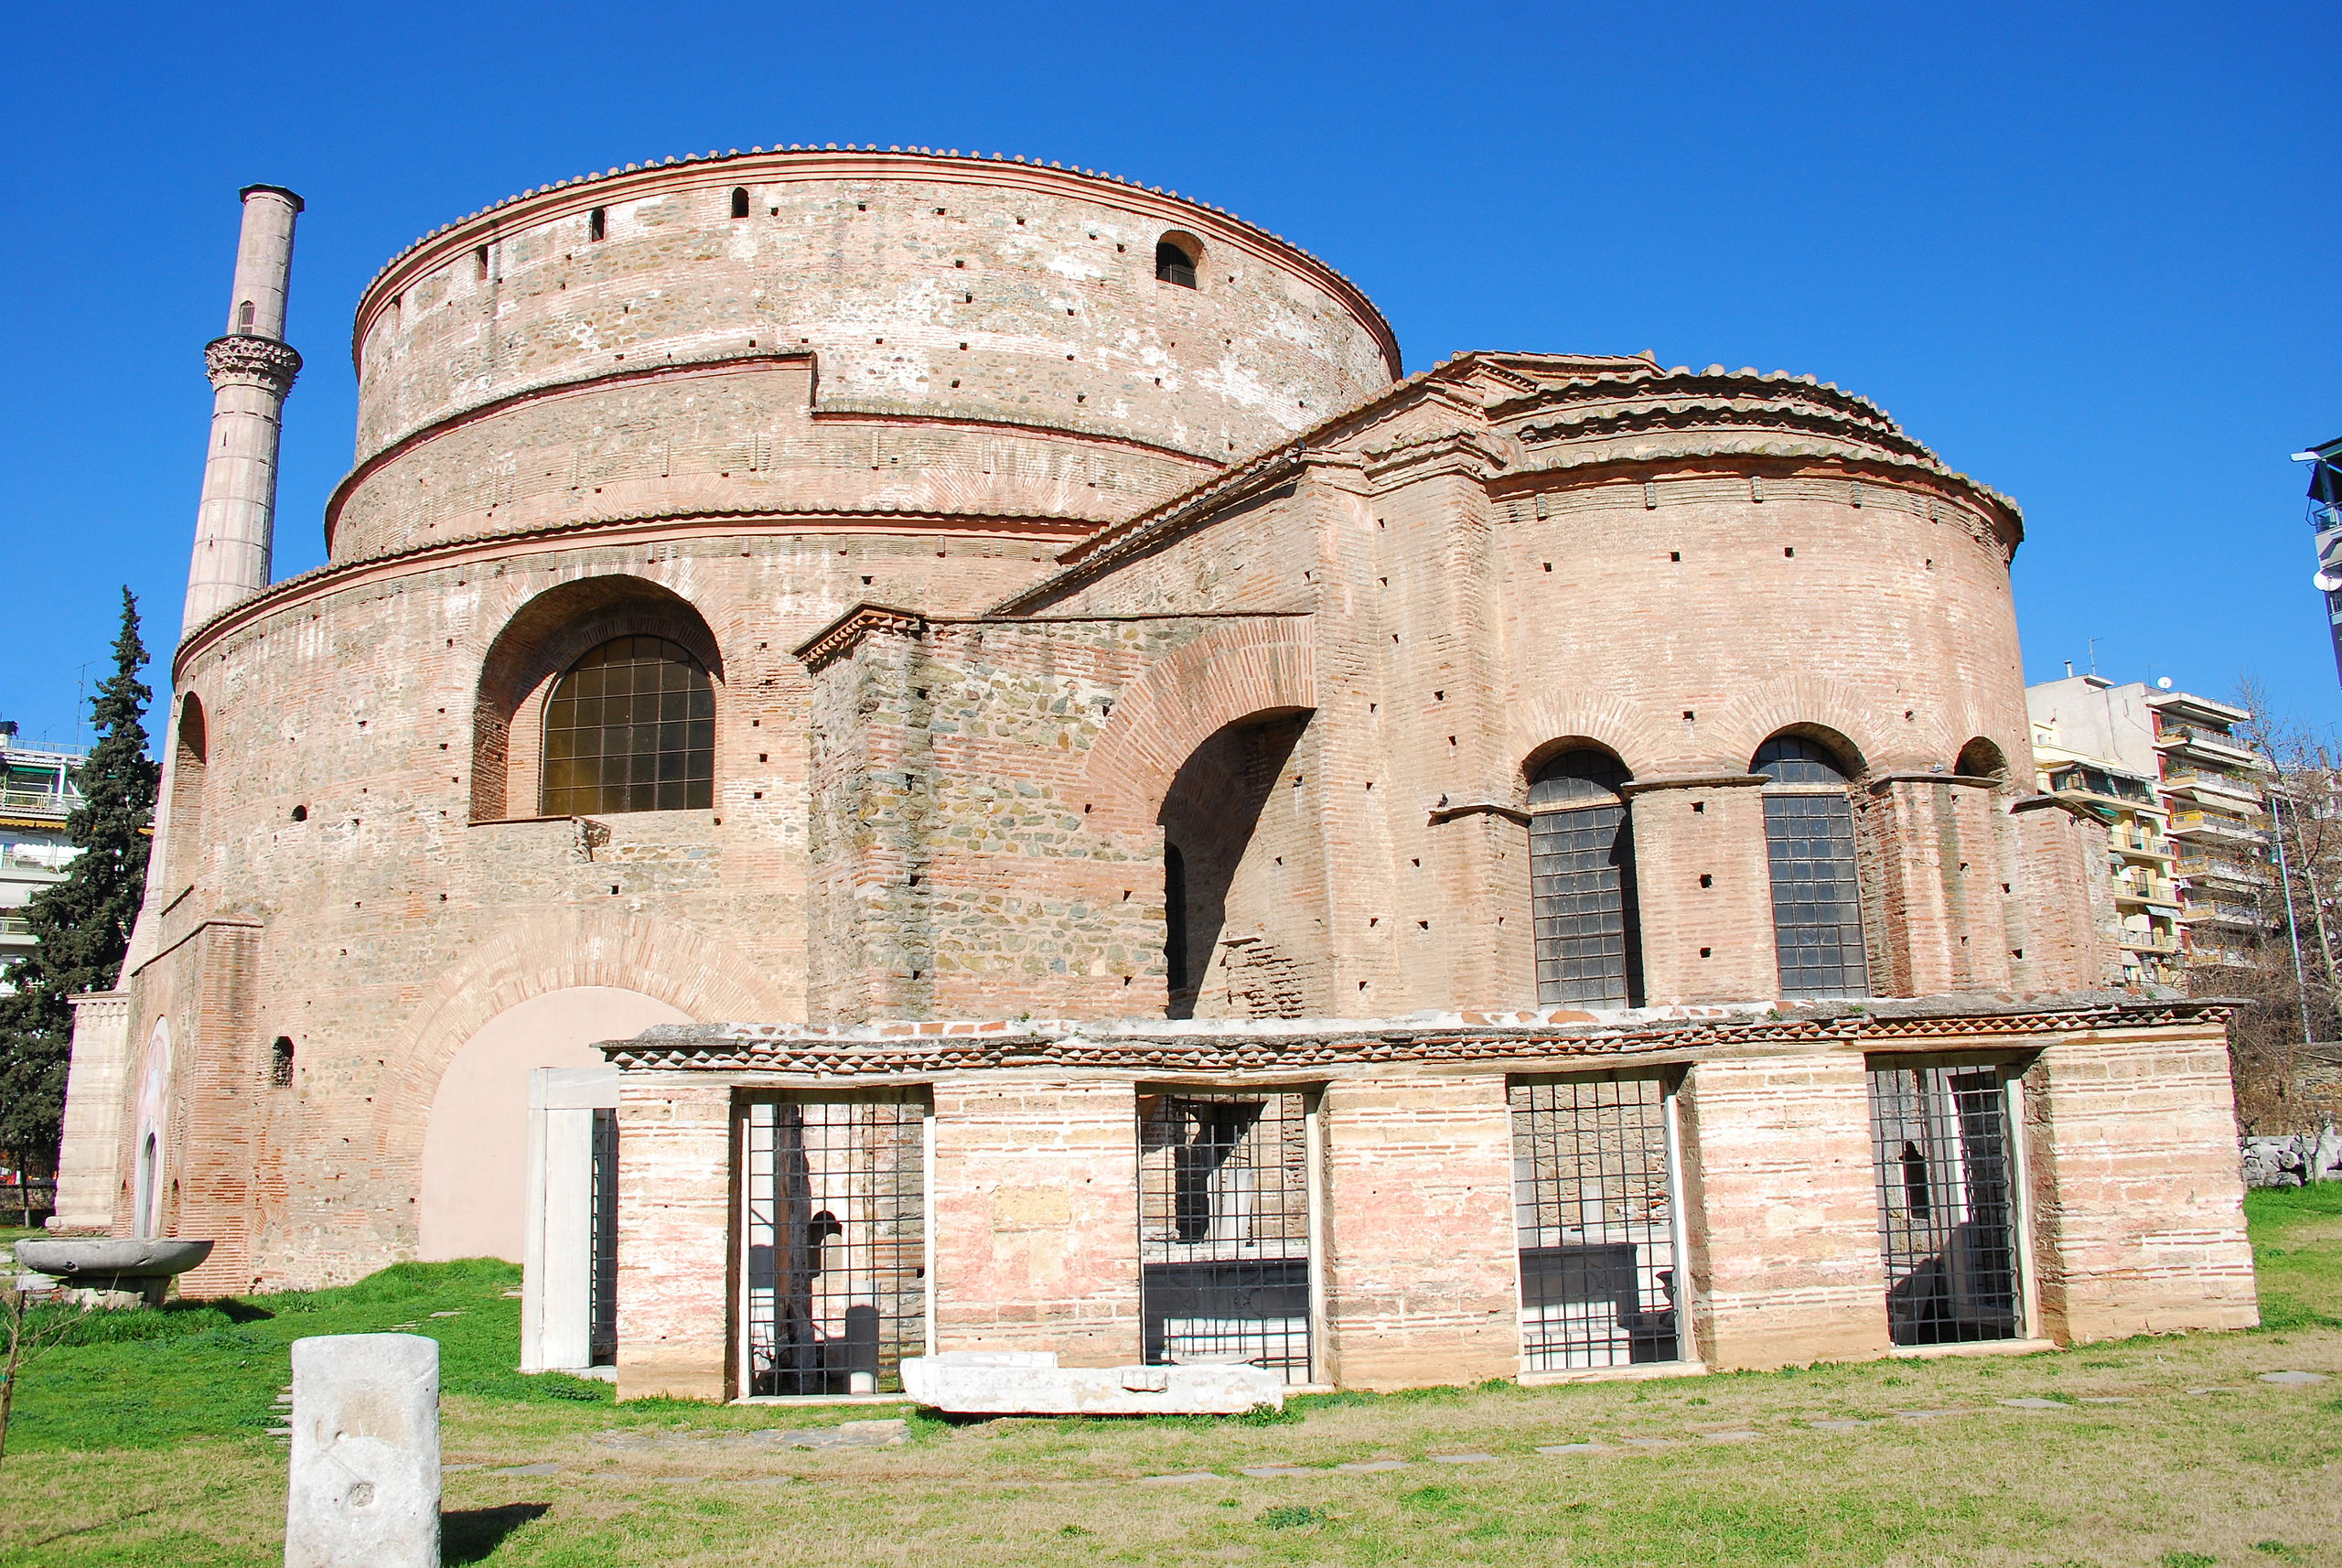
\includegraphics[width=0.52\textwidth]{figures/rotundagalerius.jpg}
	\hspace{0.2cm}
	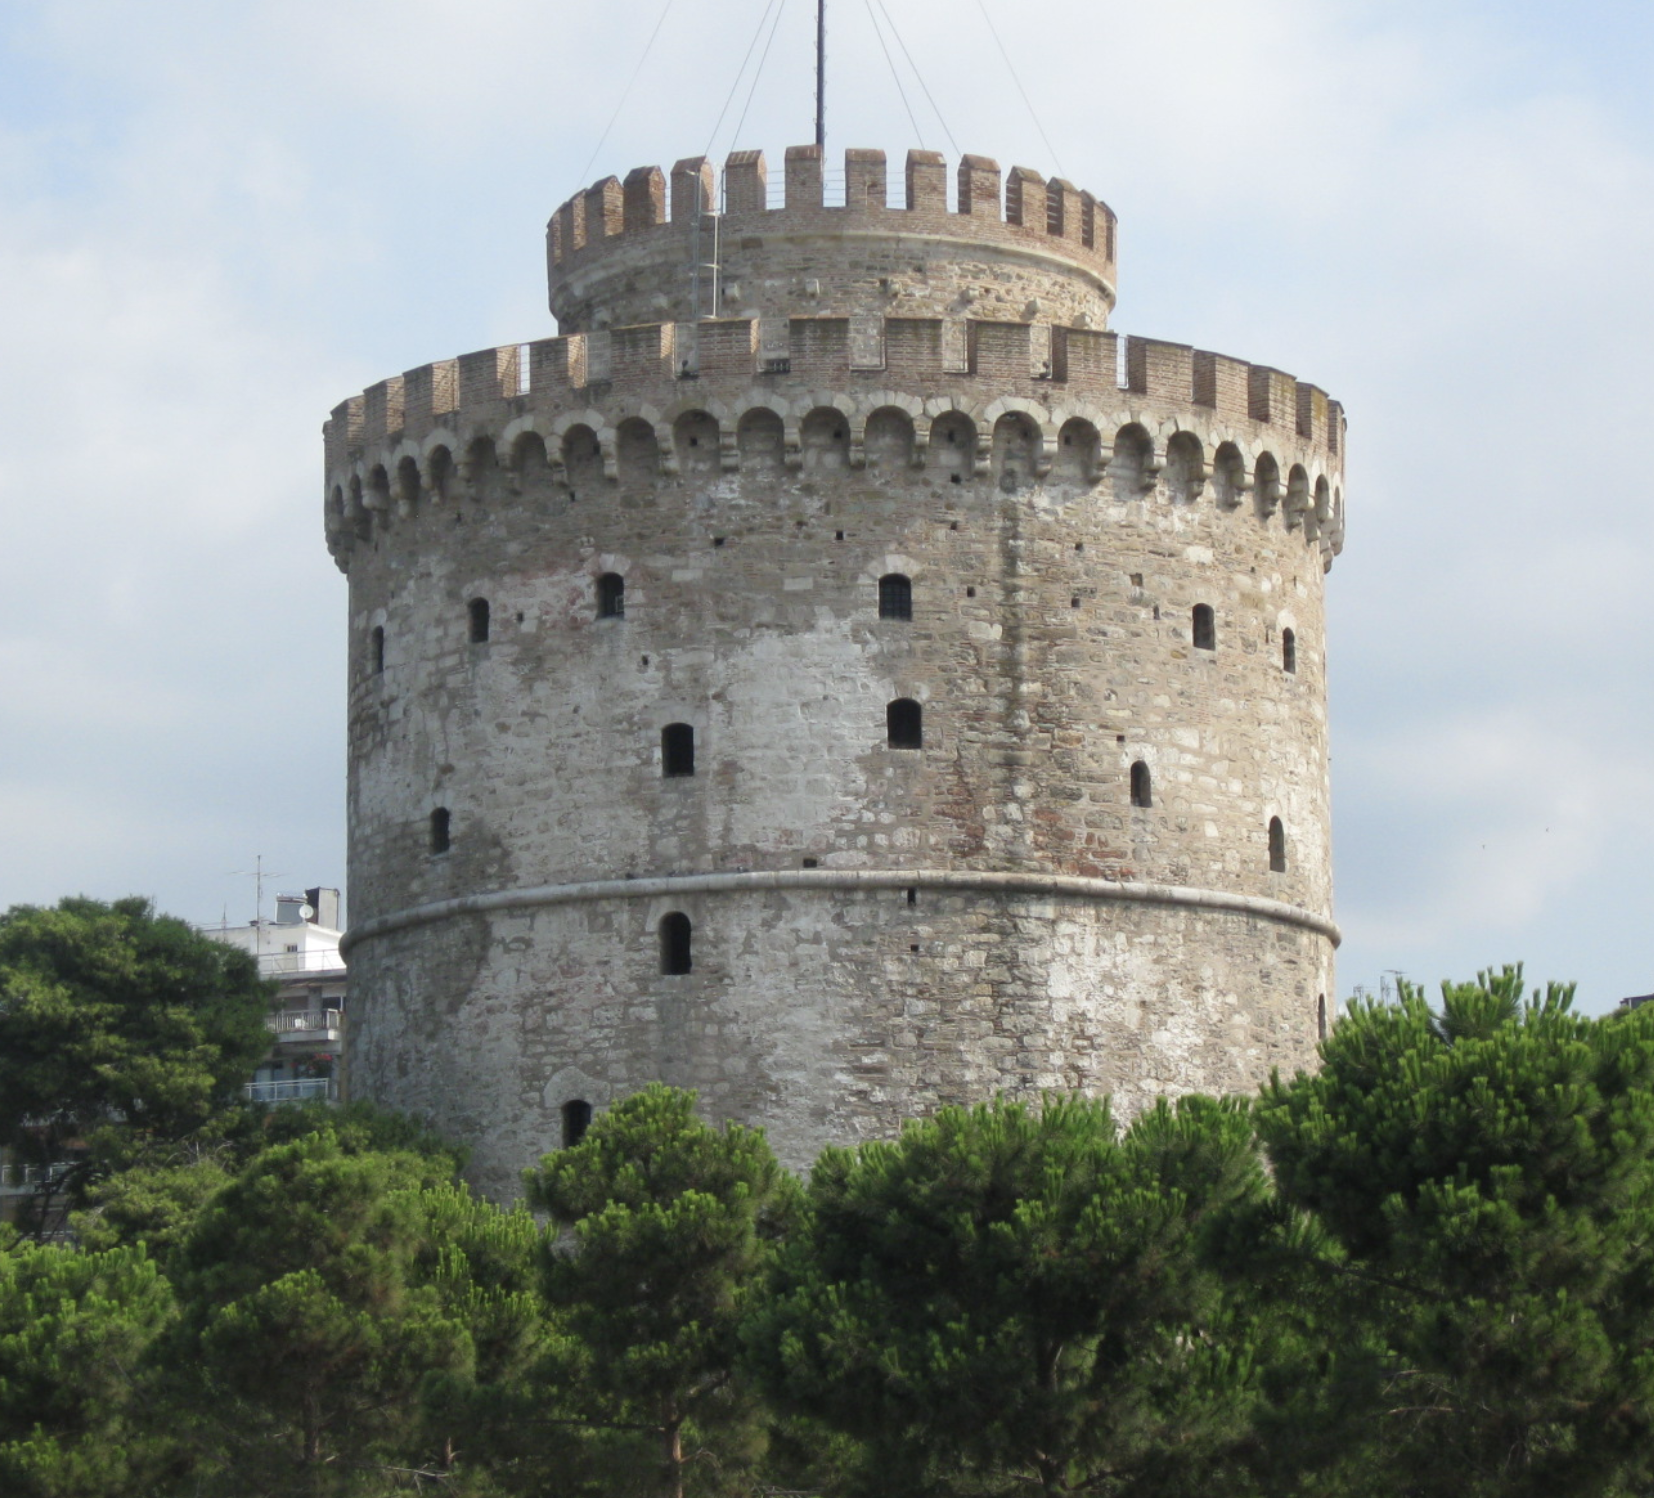
\includegraphics[width=0.42\textwidth]{figures/whitetower.png}
	
	
	\footnotesize
\textit{Source: Wikipedia}


}


\sframe{Modeling urban growth}{

% We will switch to shorter time scales, but still remain at macroscopic and mesoscopic scales.

% Understanding patterns of growth for cities is a crucial issue for its practical and policy implications e.g. regarding sustainability, but also from a theoretical point of view regarding the validation of theories for urban systems.


\centering

% meso / micro - macro

\begin{columns}
	\begin{column}{0.5\textwidth}
		Macroscopic urban system
		\medskip
		%\centering
		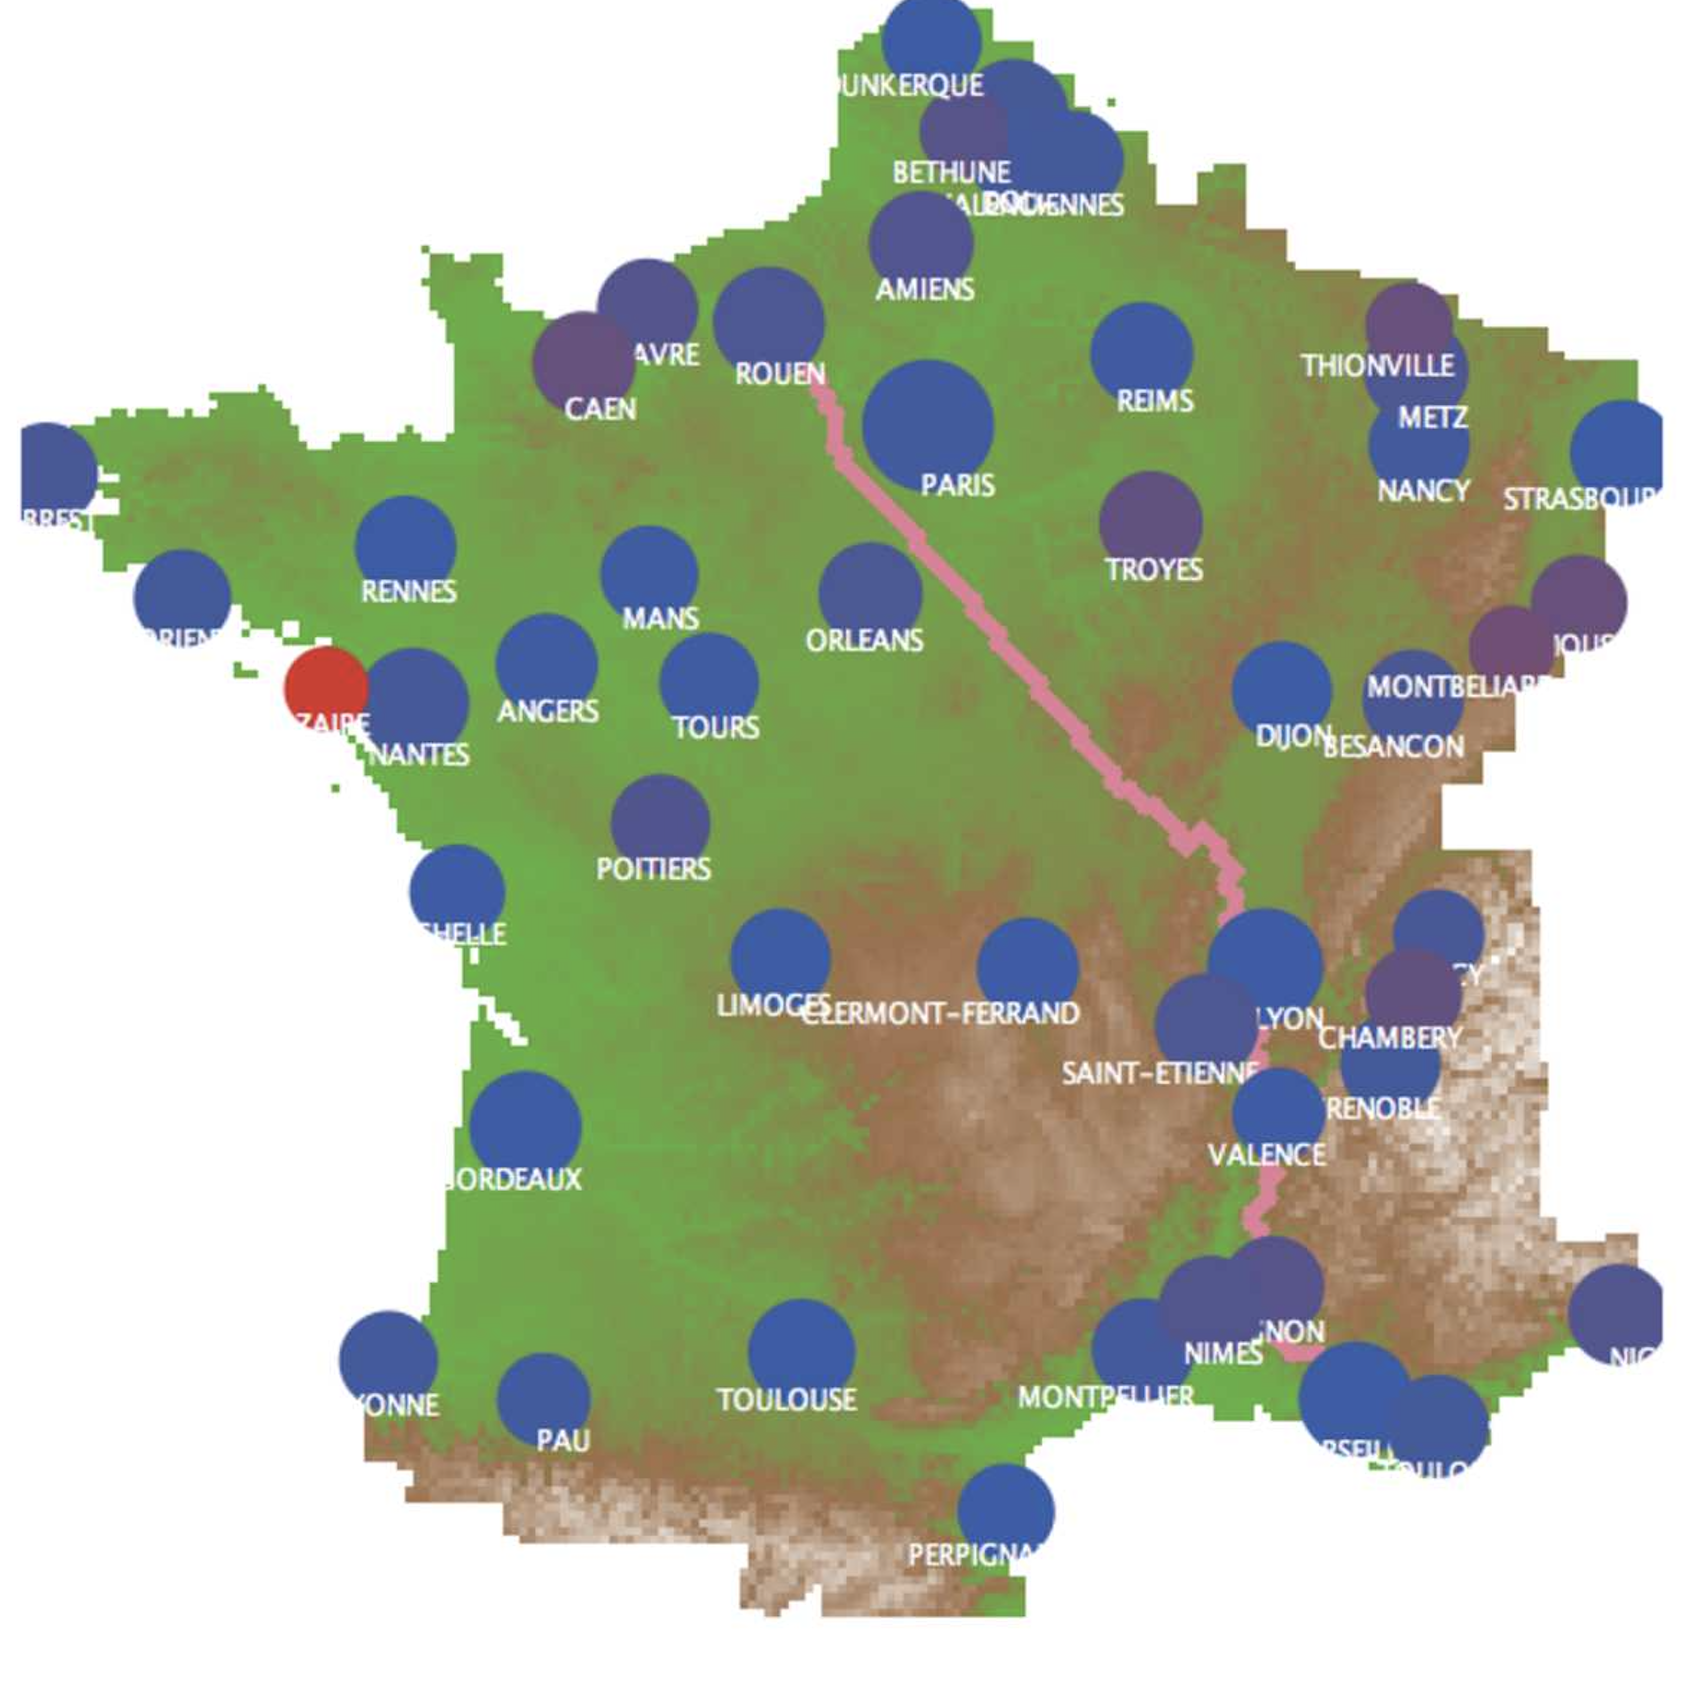
\includegraphics[width=\textwidth]{figures/macrogrowth.png}
		\footnotesize
		\justify
		Raimbault, J. (2018). Indirect evidence of network effects in a system of cities. \textit{Environment and Planning B: Urban Analytics and City Science}, 2399808318774335.
		\nocite{raimbault2018indirect}
	\end{column}
	\begin{column}{0.5\textwidth}
		Mesoscopic territorial systems
		\medskip
		%\centering
		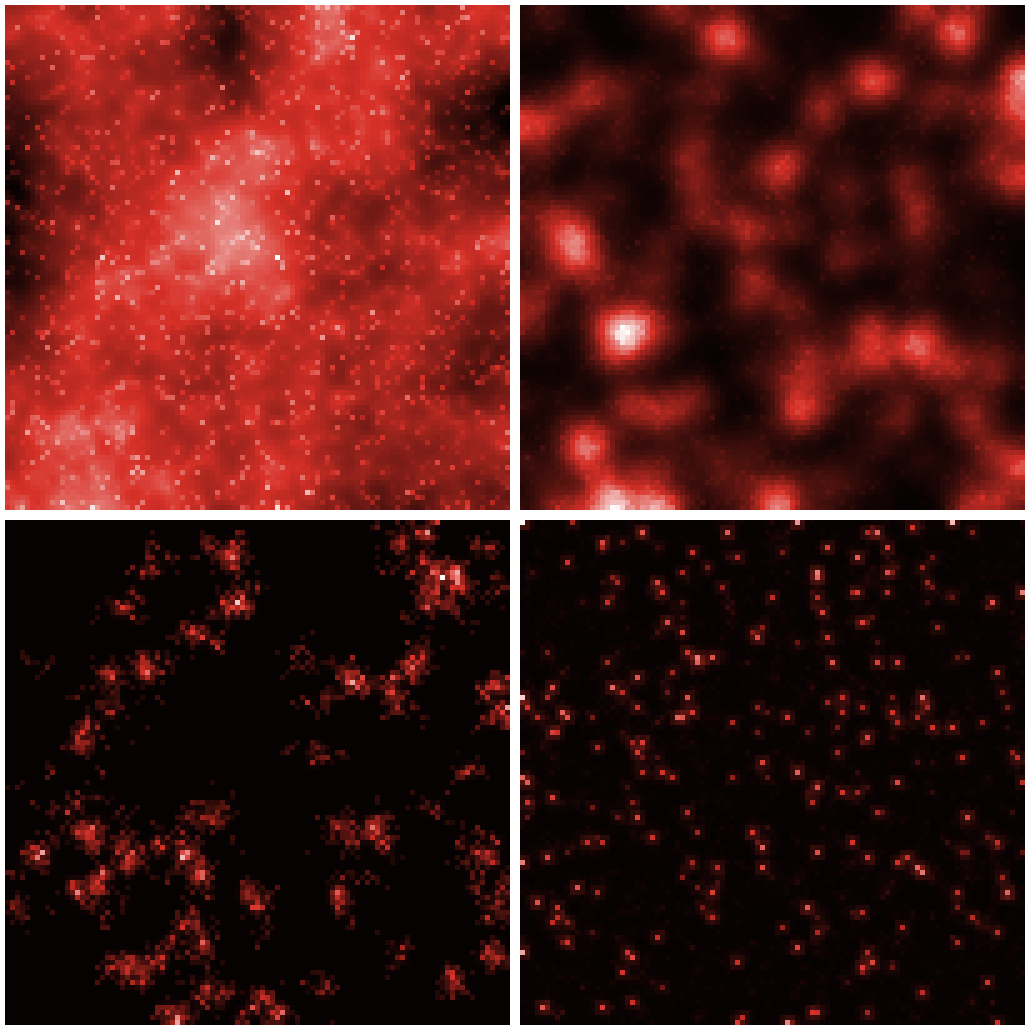
\includegraphics[width=\textwidth]{figures/mesogrowth.png}
		
		\footnotesize
		\justify
		Raimbault, J. (2018). Calibration of a density-based model of urban morphogenesis. PloS one, 13(9), e0203516.
		\nocite{raimbault2018calibration}
	\end{column}
\end{columns}



}


\sframe{An evolutionary urban theory}{

% A particular entry is taken by the Evolutive Urban Theory [1] which postulates interactions between cities as main drivers of their growth.

From \cite{pumain1997pour} to \cite{pumain2018evolutionary}: systems of cities as co-evolutive systems in which interactions are crucial

\centering

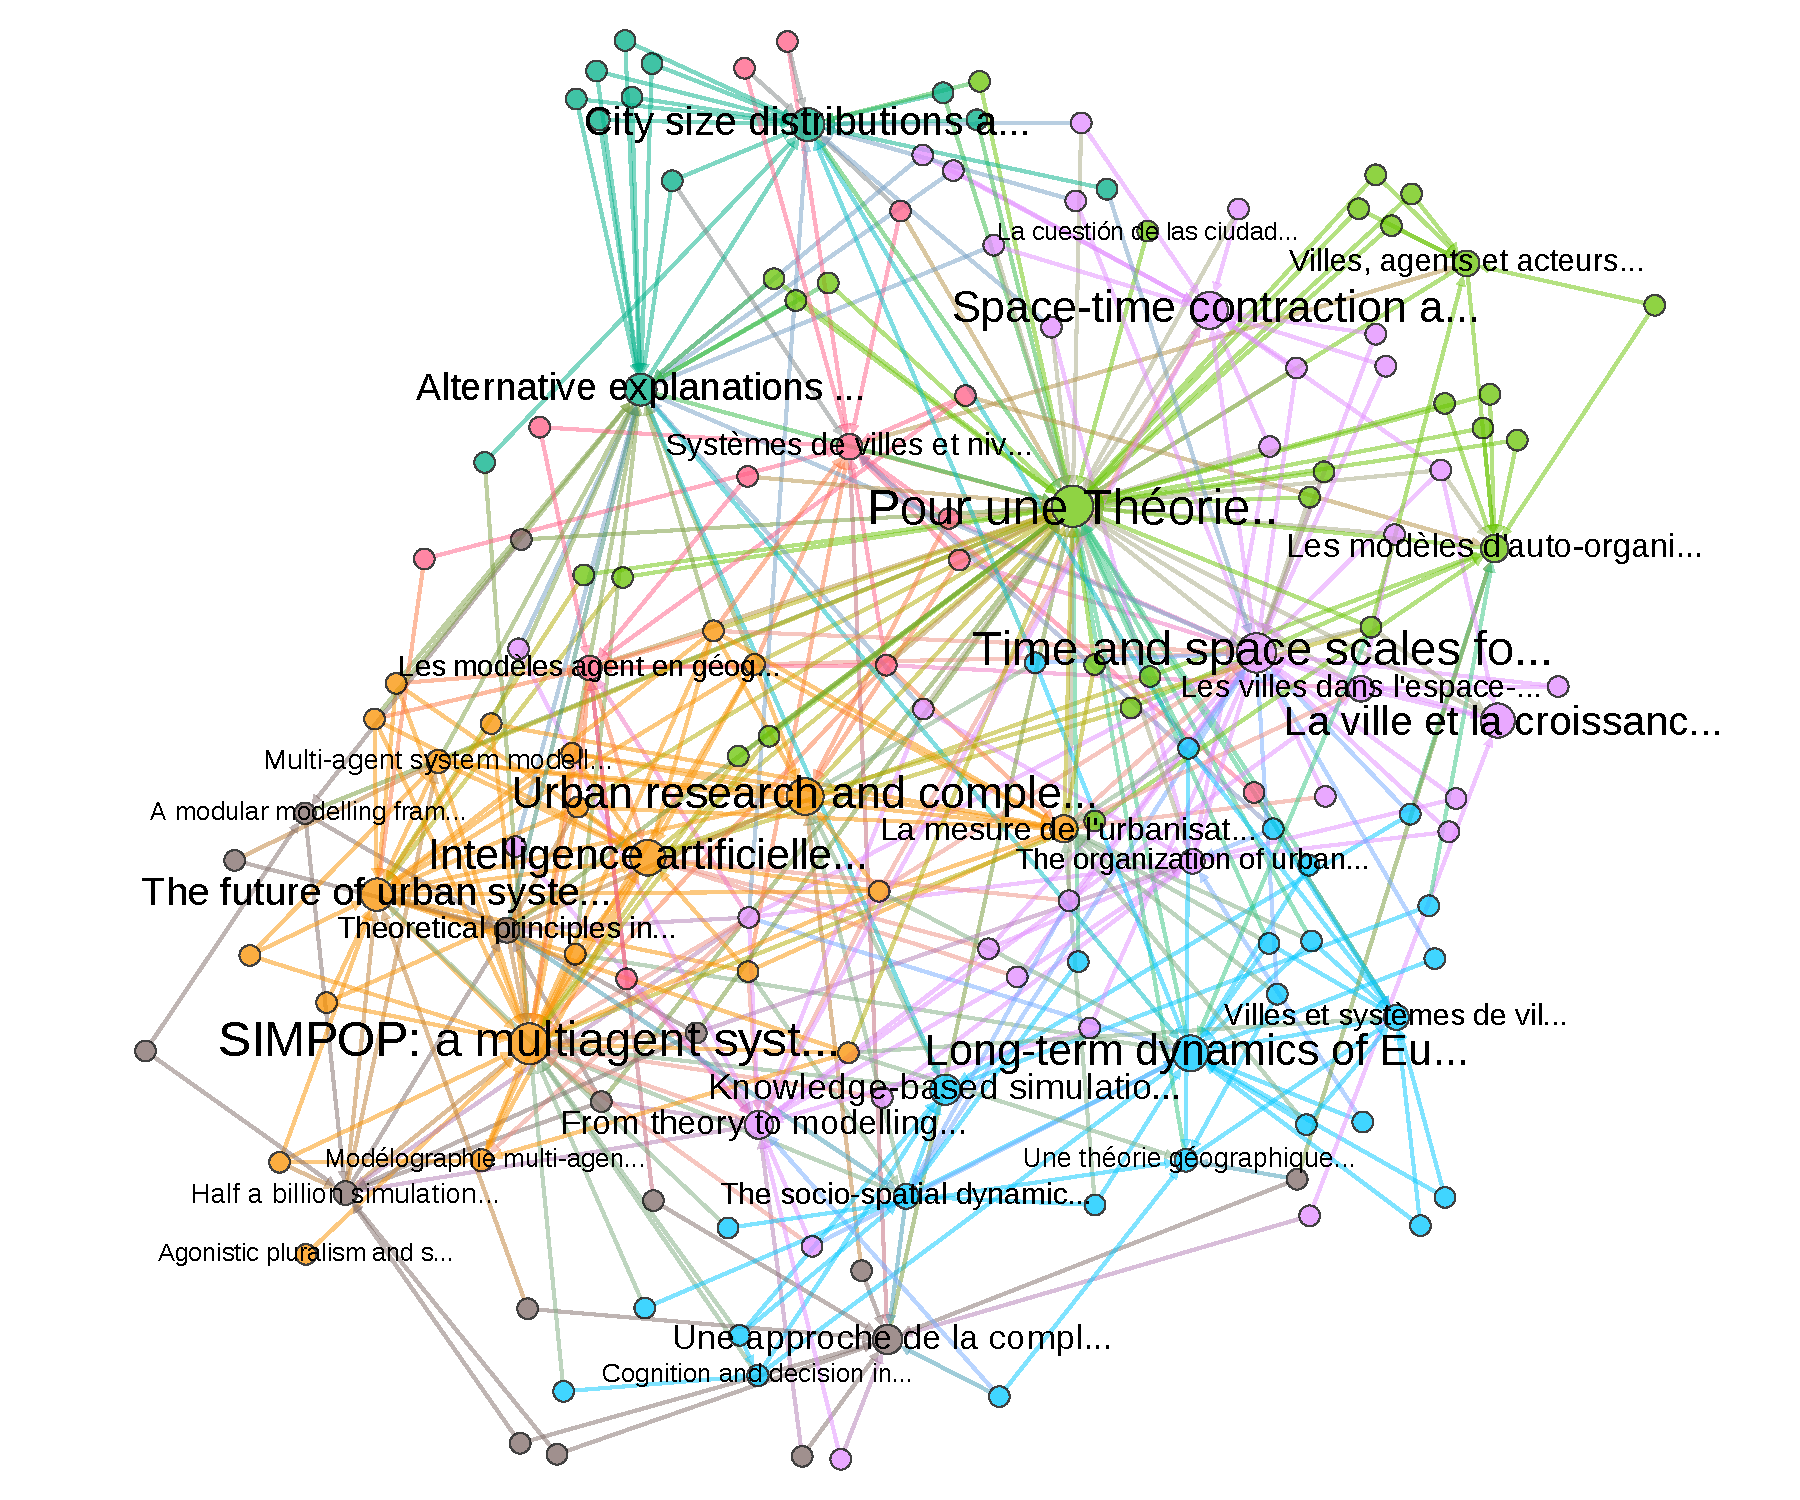
\includegraphics[height=0.7\textheight]{figures/evolurbantheory.pdf}

\footnotesize
\textit{\cite{raimbault2017applied} Citation network analysis of core publications in the evolutionary urban theory}

}





\sframe{Towards a systematic model comparison}{

% Within this framework, numerous concurrent models have been introduced for the evolution of systems of cities, and applied on diverse case studies, but there is to the best of our knowledge no systematic comparison of performances across models and application cases. This contribution makes a first step towards such a systematic benchmark.


\justify

$\rightarrow$ several models in this context have been introduced, but never compared (e.g. in terms of explanative power)

\medskip

$\rightarrow$ multidimensionality of urban systems and the potential complementarity between very different processes

% research question

% before coupling models, benchmarking them !

\bigskip
\bigskip

\textbf{Research objective : } \textit{Benchmark interaction models for systems of cities developed in the frame of the evolutionary urban theory, on several comparable systems of cities.}

}





\sframe{Urban systems interaction models}{

%  We consider simple models simulating population of cities only, but including heterogenous underlying processes and assumptions. More precisely, we compare (i) the Favaro-Pumain model for the diffusion of innovation [2]; (ii) the Marius multi-model based on economic exchanges [3]; and (iii) a model including flows within abstract physical networks parametrized on elevation data [4].

%\centering
\justify

Comparison of three approaches based on the evolutionary urban theory \cite{pumain1997pour} capturing different dimensions of urban systems:

\bigskip

\begin{itemize}
	\item The Favaro-Pumain model for the diffusion of innovation \cite{favaro2011gibrat}
	\item The Marius model family based on economic exchanges \cite{cottineau2014evolution}
	\item An interaction model including physical transportation networks \cite{raimbault2018indirect}
\end{itemize}

}


\sframe{Description of models}{

% increasing complexity for the presentation of models

\begin{columns}
	\begin{column}{0.33\textwidth}
		\textbf{Network interaction model}
		
		\medskip

		\begin{itemize}
			\item Endogenous growth
			\item Interactions inducing growth through gravity potential
			\item Static physical network taken into account (geographical shortest path with topography)
		\end{itemize}
		
	\end{column}
	\vrule{}
	\begin{column}{0.33\textwidth}
		%\vspace{-1cm}
		\textbf{Favaro-Pumain model}
		
		\medskip
		
		\begin{itemize}
			\item Endogenous growth
			\item Innovation emerge and diffuse in cities
			\item Growth rates adapted according to utility of innovation and level of adaptation
		\end{itemize}
			
	\end{column}
	\vrule{}
	\begin{column}{0.33\textwidth}
		\textbf{Marius model}
		
		\medskip
		
		\begin{itemize}
			\item Cities produce economic goods
			\item Economic exchanges are estimated according to gravity flows
			\item Populations grow depending on final economic balances
		\end{itemize}

		
	\end{column}
\end{columns}





}





\sframe{Datasets}{

% These models are calibrated on a large scale harmonized dataset [5] including the European, former Soviet Union, Chinese, Brazilian, South-African, Indian and USA systems of cities on a time period covering 1960-2010.

%\centering

% geodivercity harmonization of datasets

\justify

\textbf{Dataset}

Harmonized dataset, explored in particular by \cite{pumain2015multilevel} (built in the context of Geodivercity ERC): Urban systems for Europe, United States, Brazil, China, India, South Africa, Russia, consistent and comparable between 1960 and 2010 each 10 years.

\bigskip

\textbf{Data preprocessing}

\begin{itemize}
	\item Remove small cities and medium-sized cities (\cite{adam2006medium} for definition of medium-sized) for scalability of simulations
	\item Shortest paths matrices (direct and taking into account topography, using the EEA world DEM) computed a priori and cached (\textit{no evolution of the network})
\end{itemize}



}



\sframe{Stylized facts}{
%\centering

% - fit distributions of growth rates
% - cluster by type of distrib ?

\textit{Population distributions mainly log-normal (75\% with KS-test, all with AIC); consistent hierarchies in time.}

\medskip

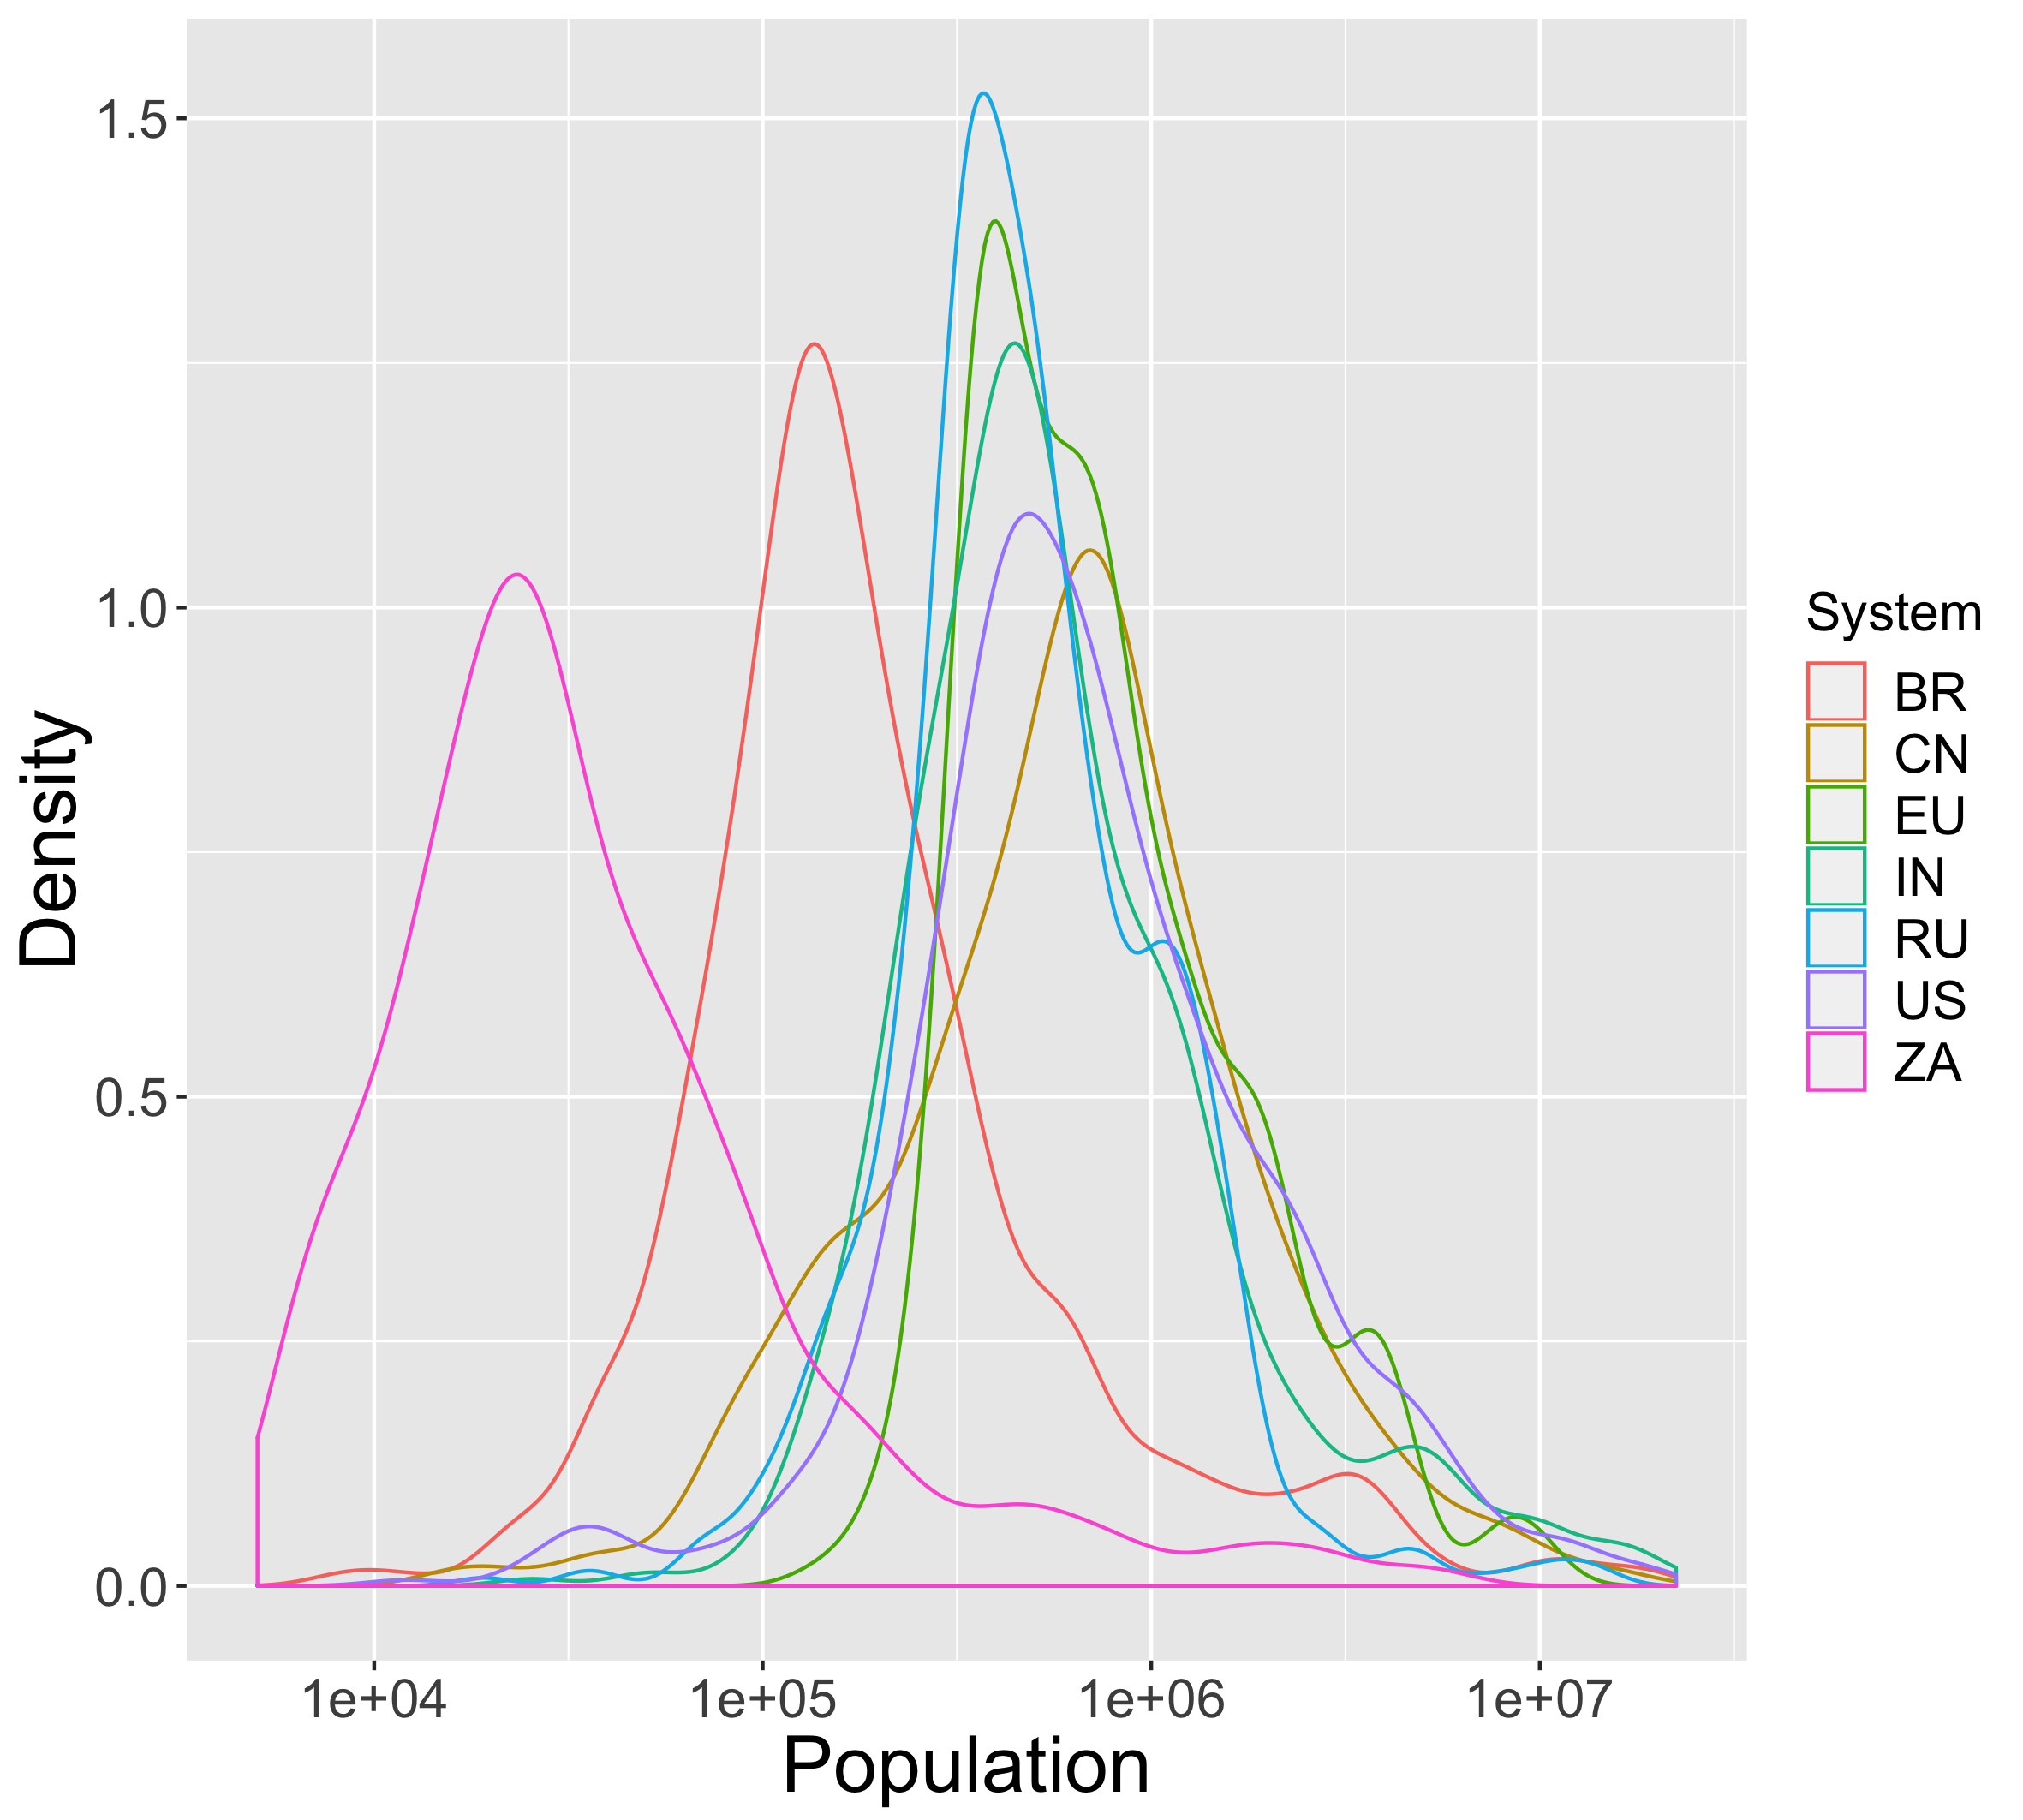
\includegraphics[width=0.49\textwidth]{figures/popdistribs.png}
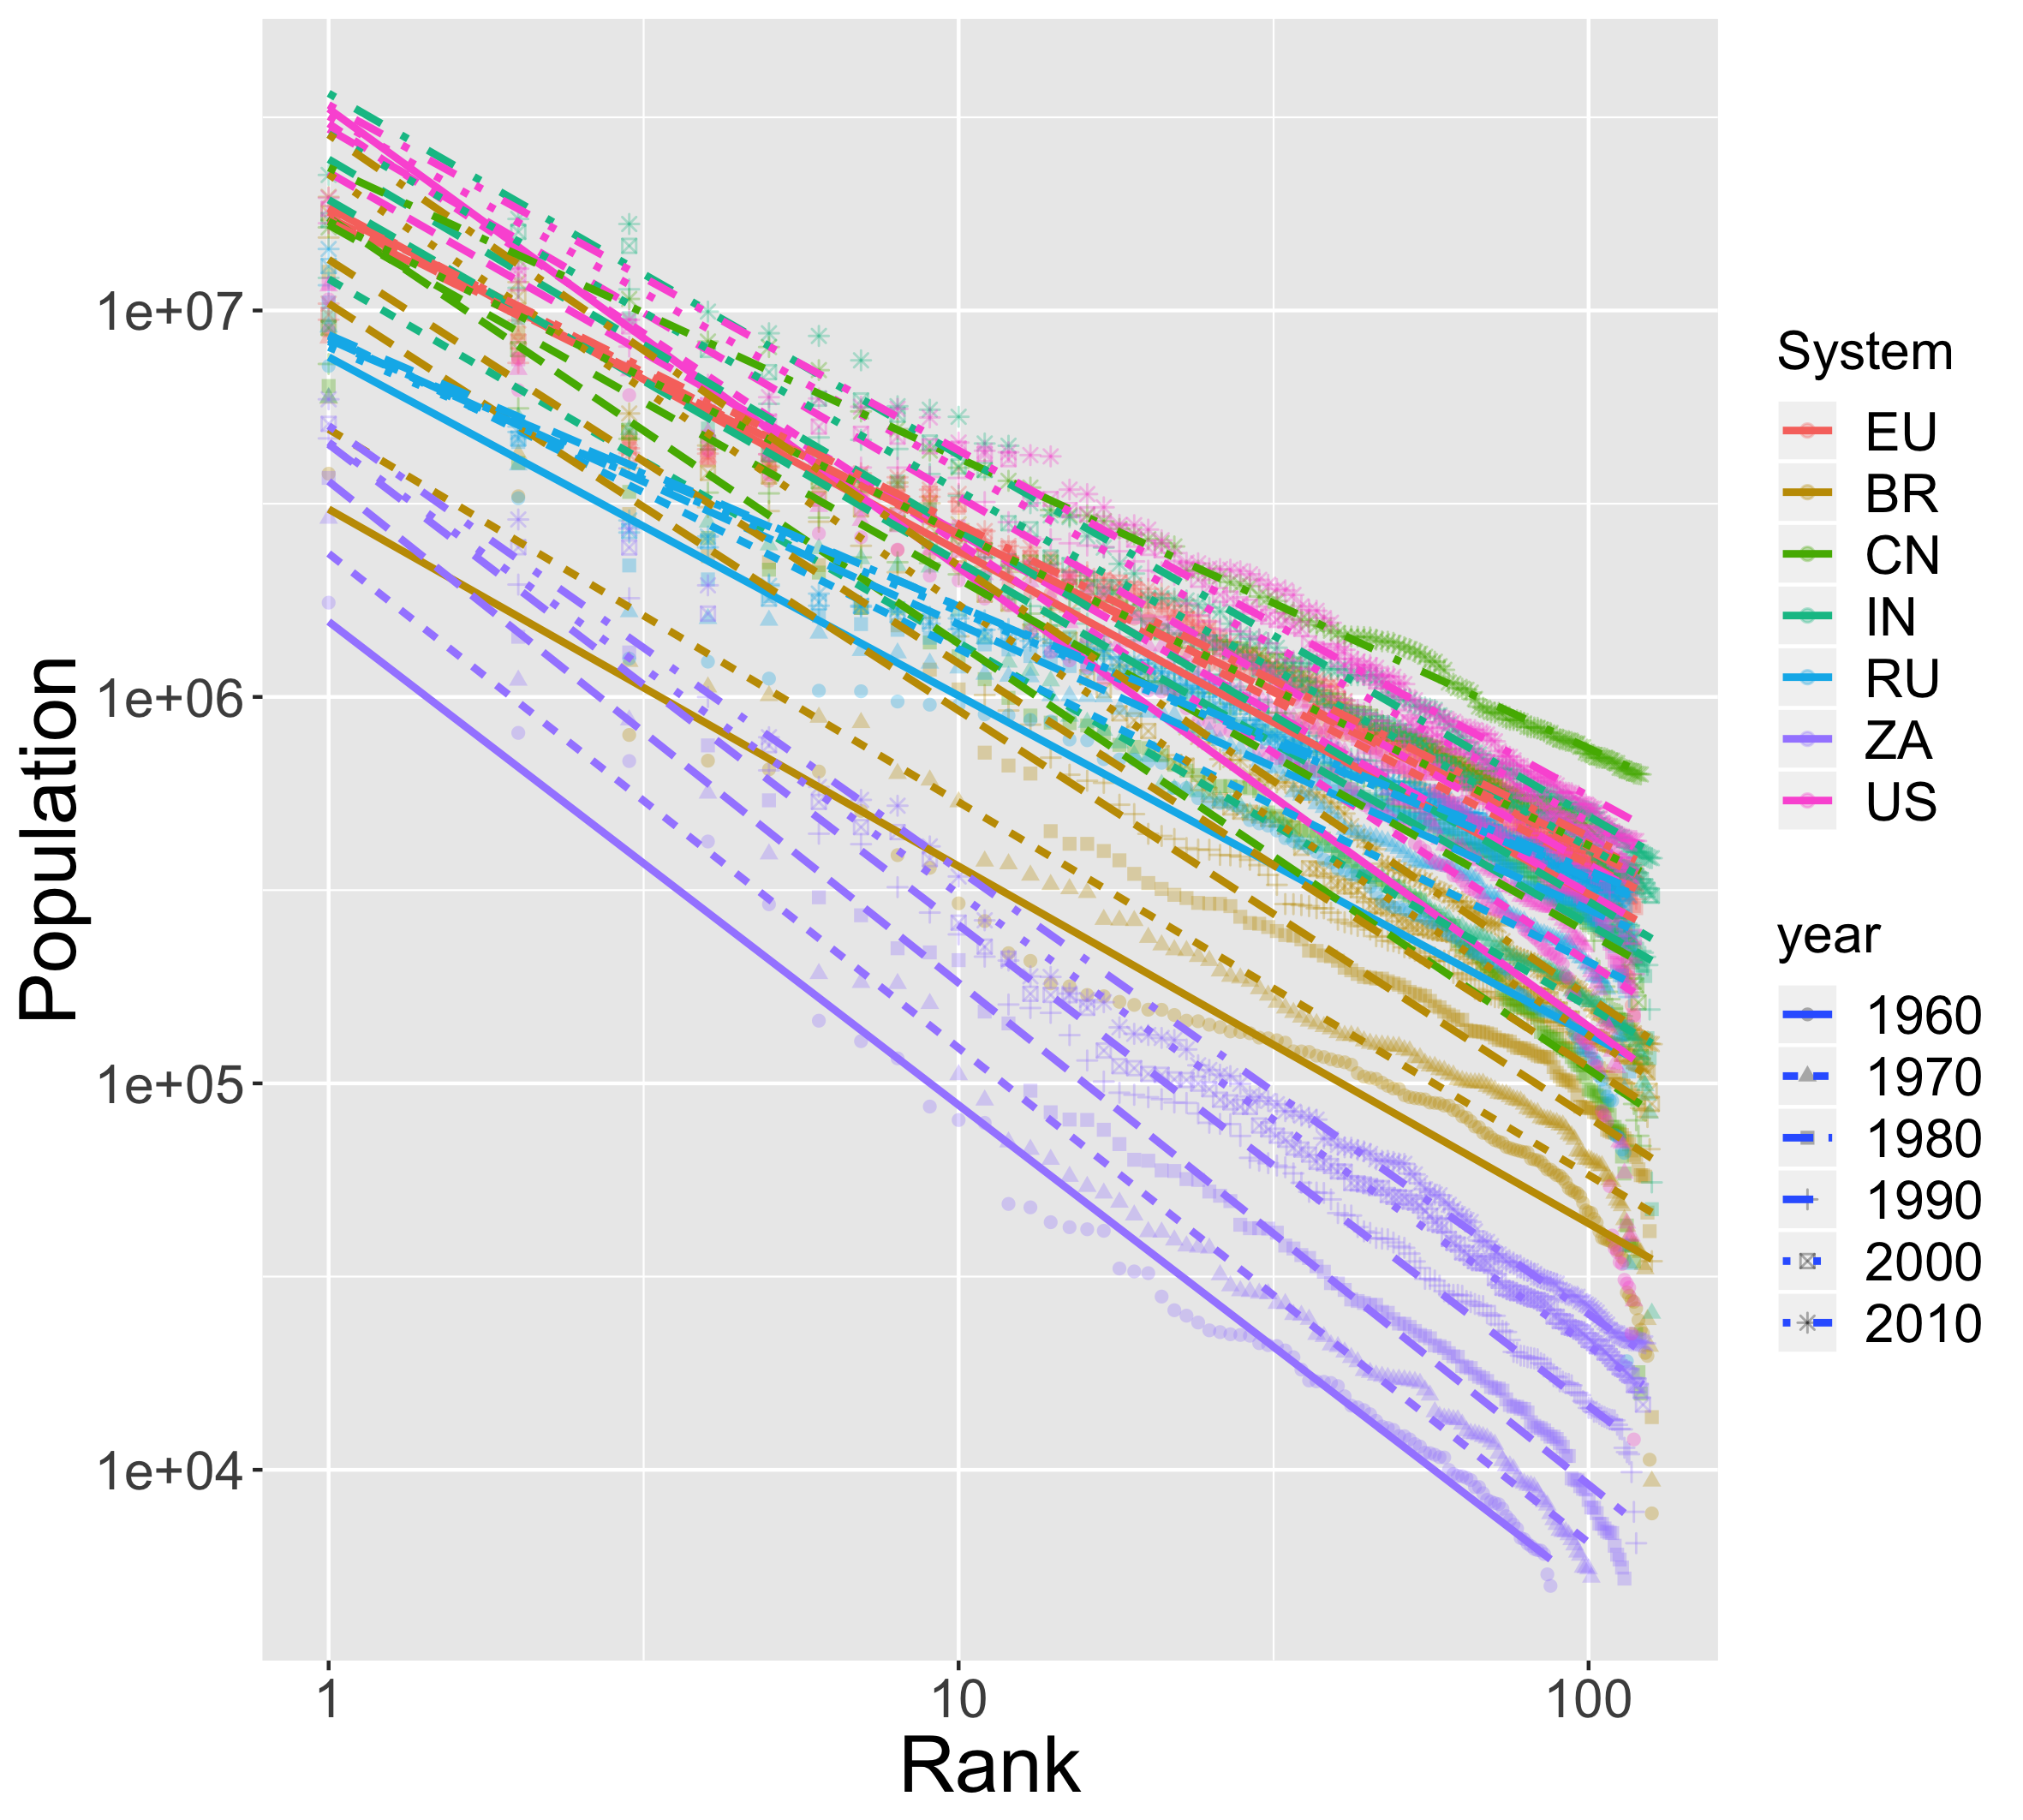
\includegraphics[width=0.49\textwidth]{figures/popranksize.png}

}

\sframe{Stylized facts}{

\textit{Growth rates distributions evolve considerably in time}

\medskip

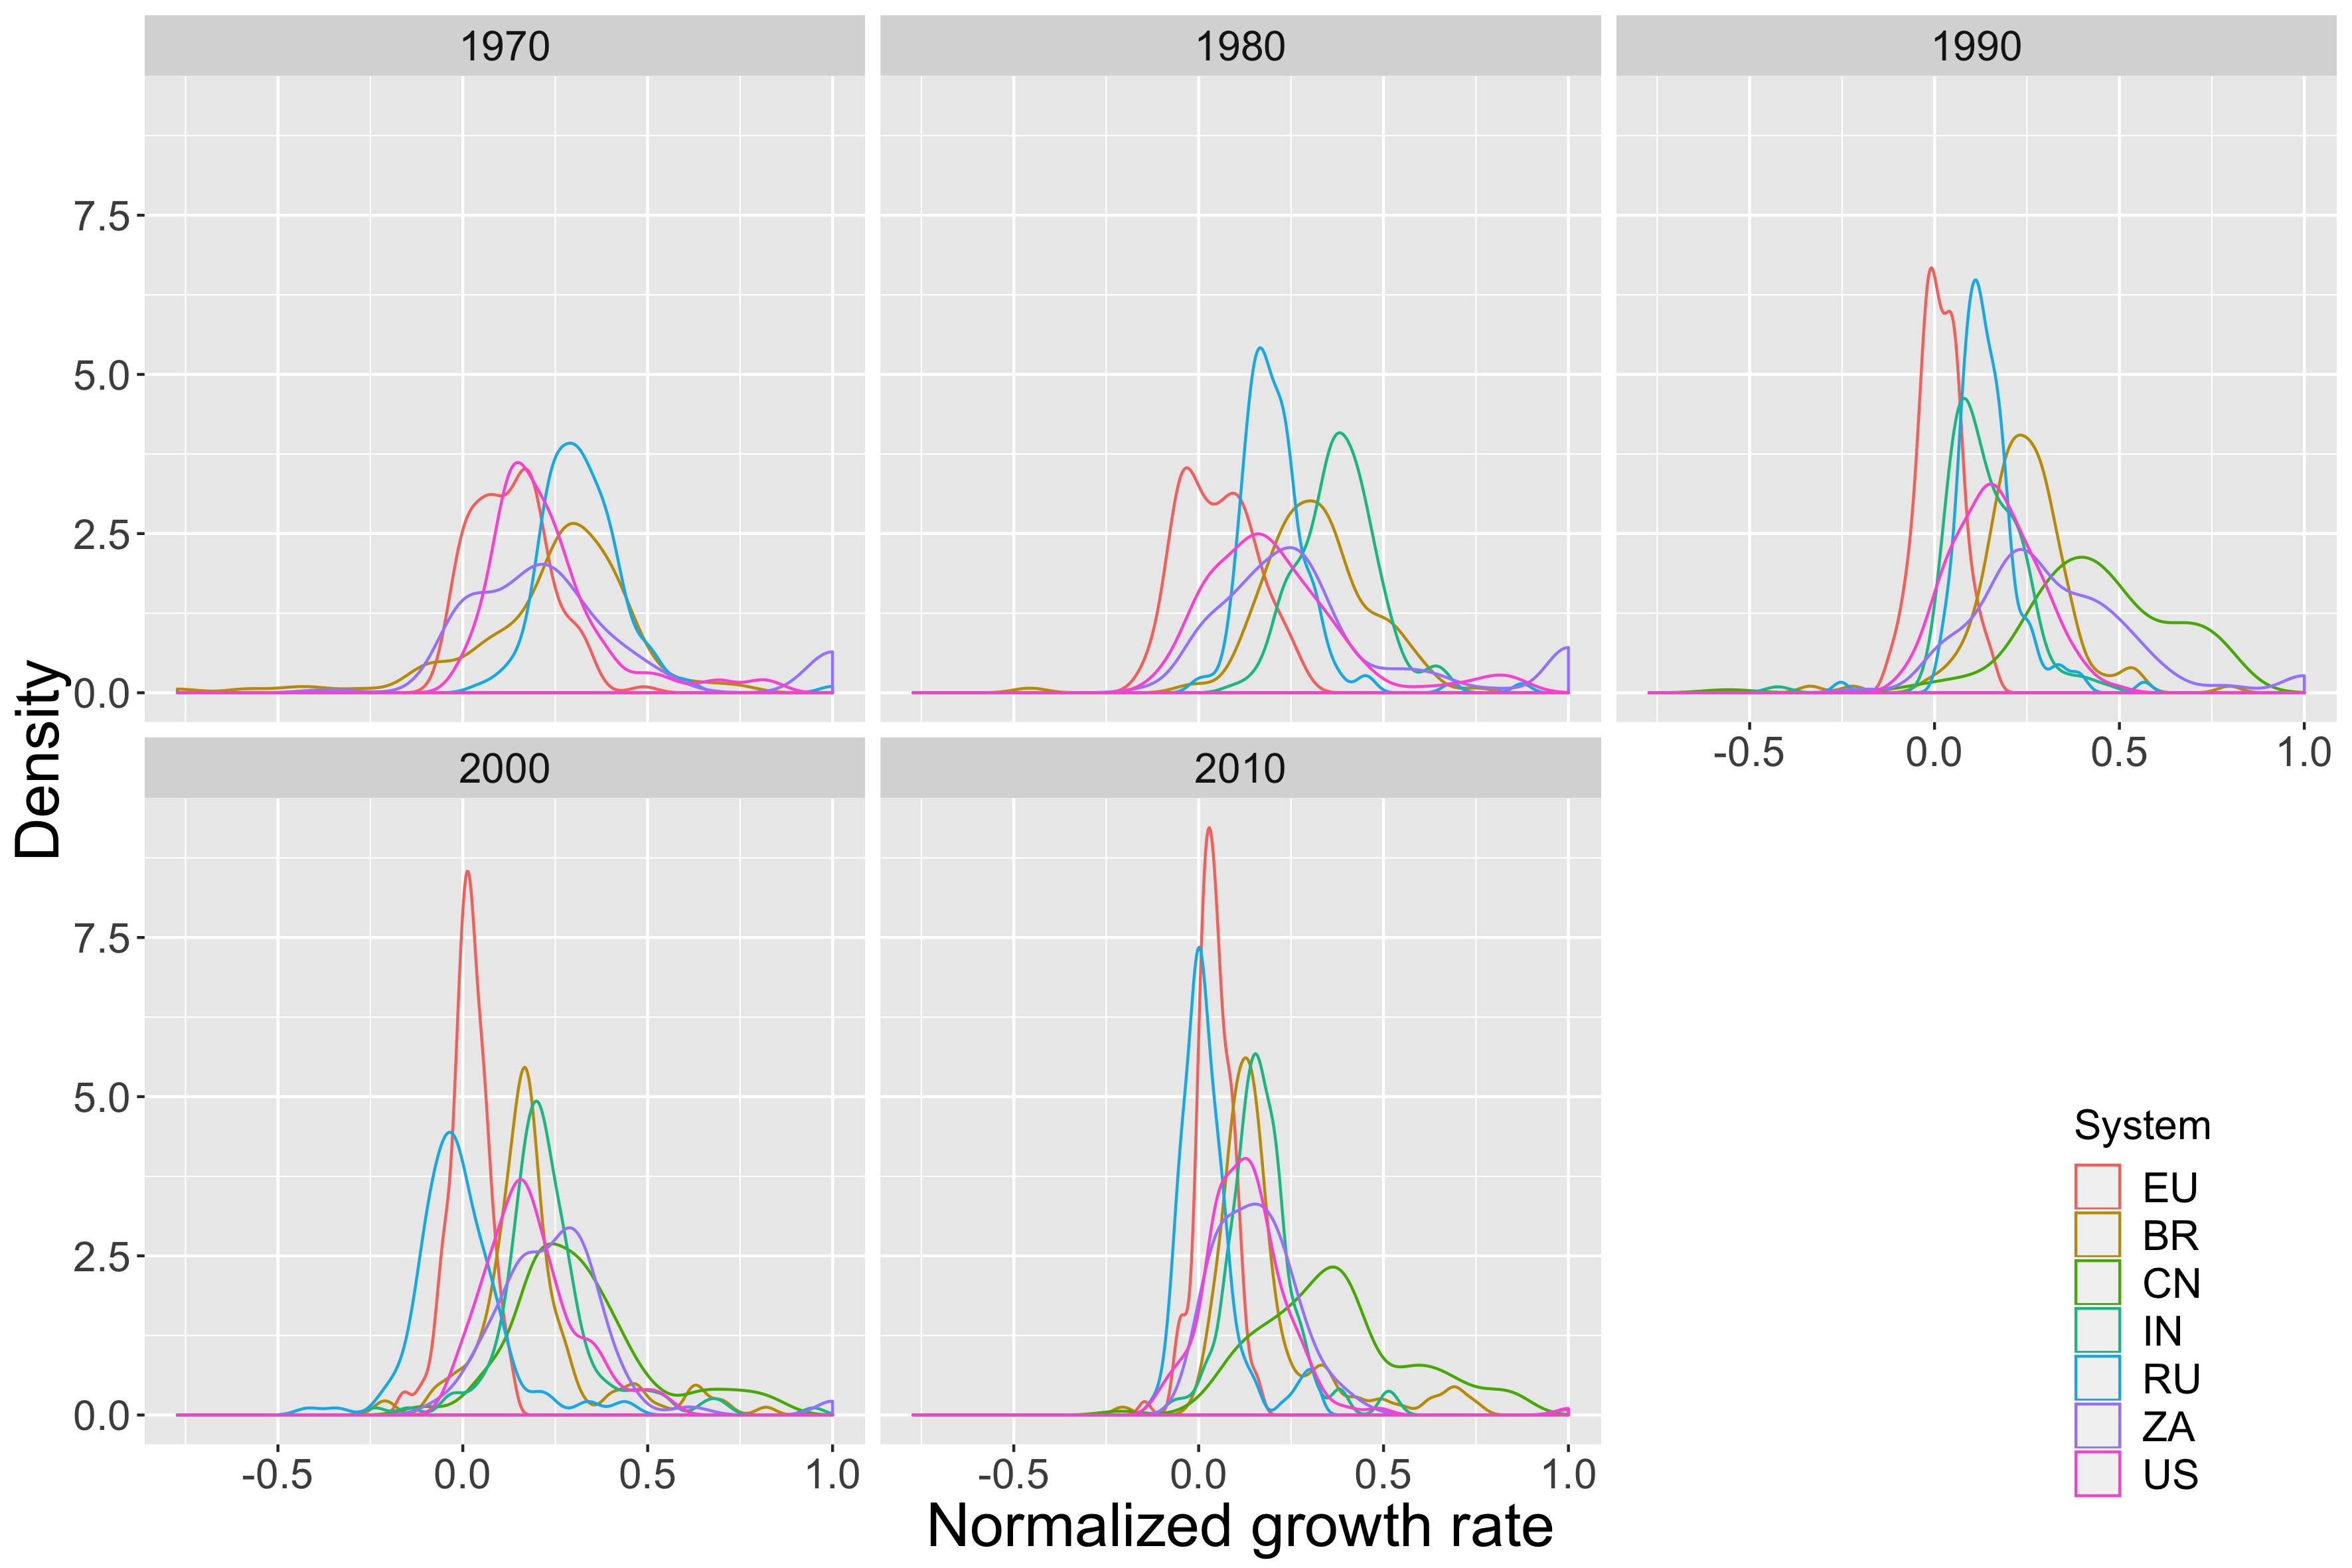
\includegraphics[width=\textwidth]{figures/growthrates_byyear.png}

}

\sframe{Stylized facts}{

\textit{Correlation as a function of distance: long-range correlations in several systems}

\medskip

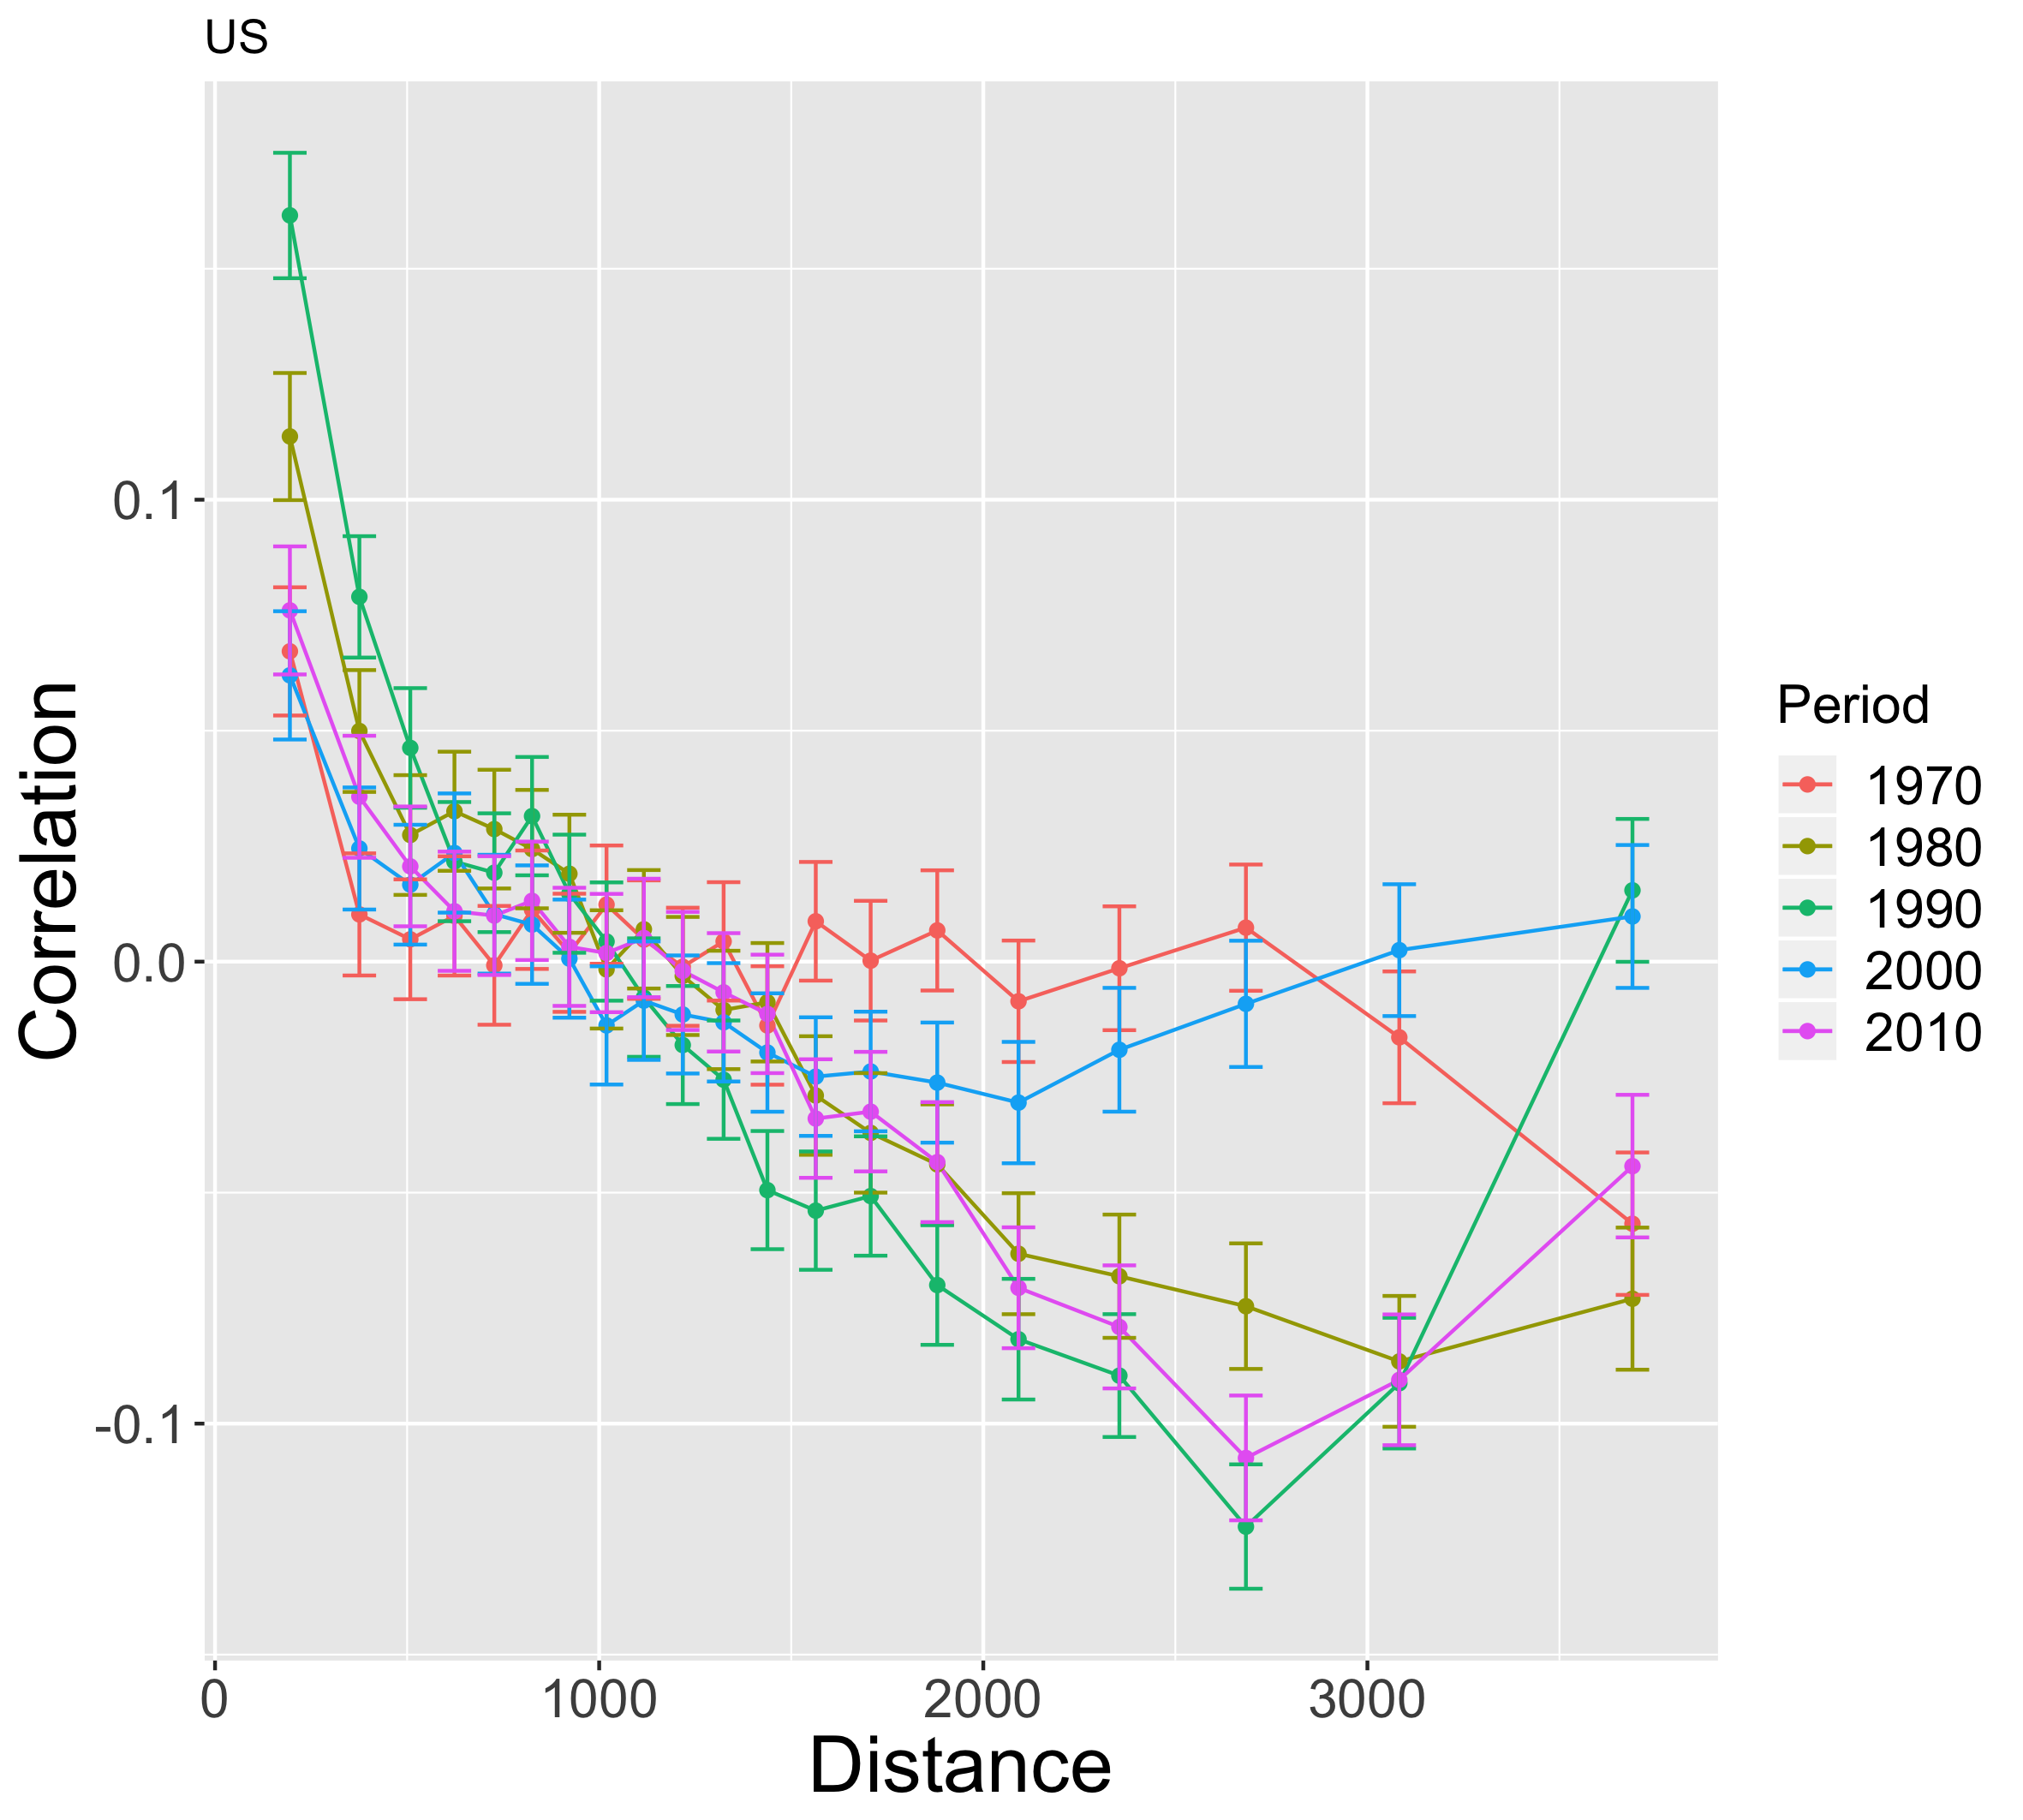
\includegraphics[width=0.49\textwidth]{figures/corrsdist_US_quantiles21_periods5.png}
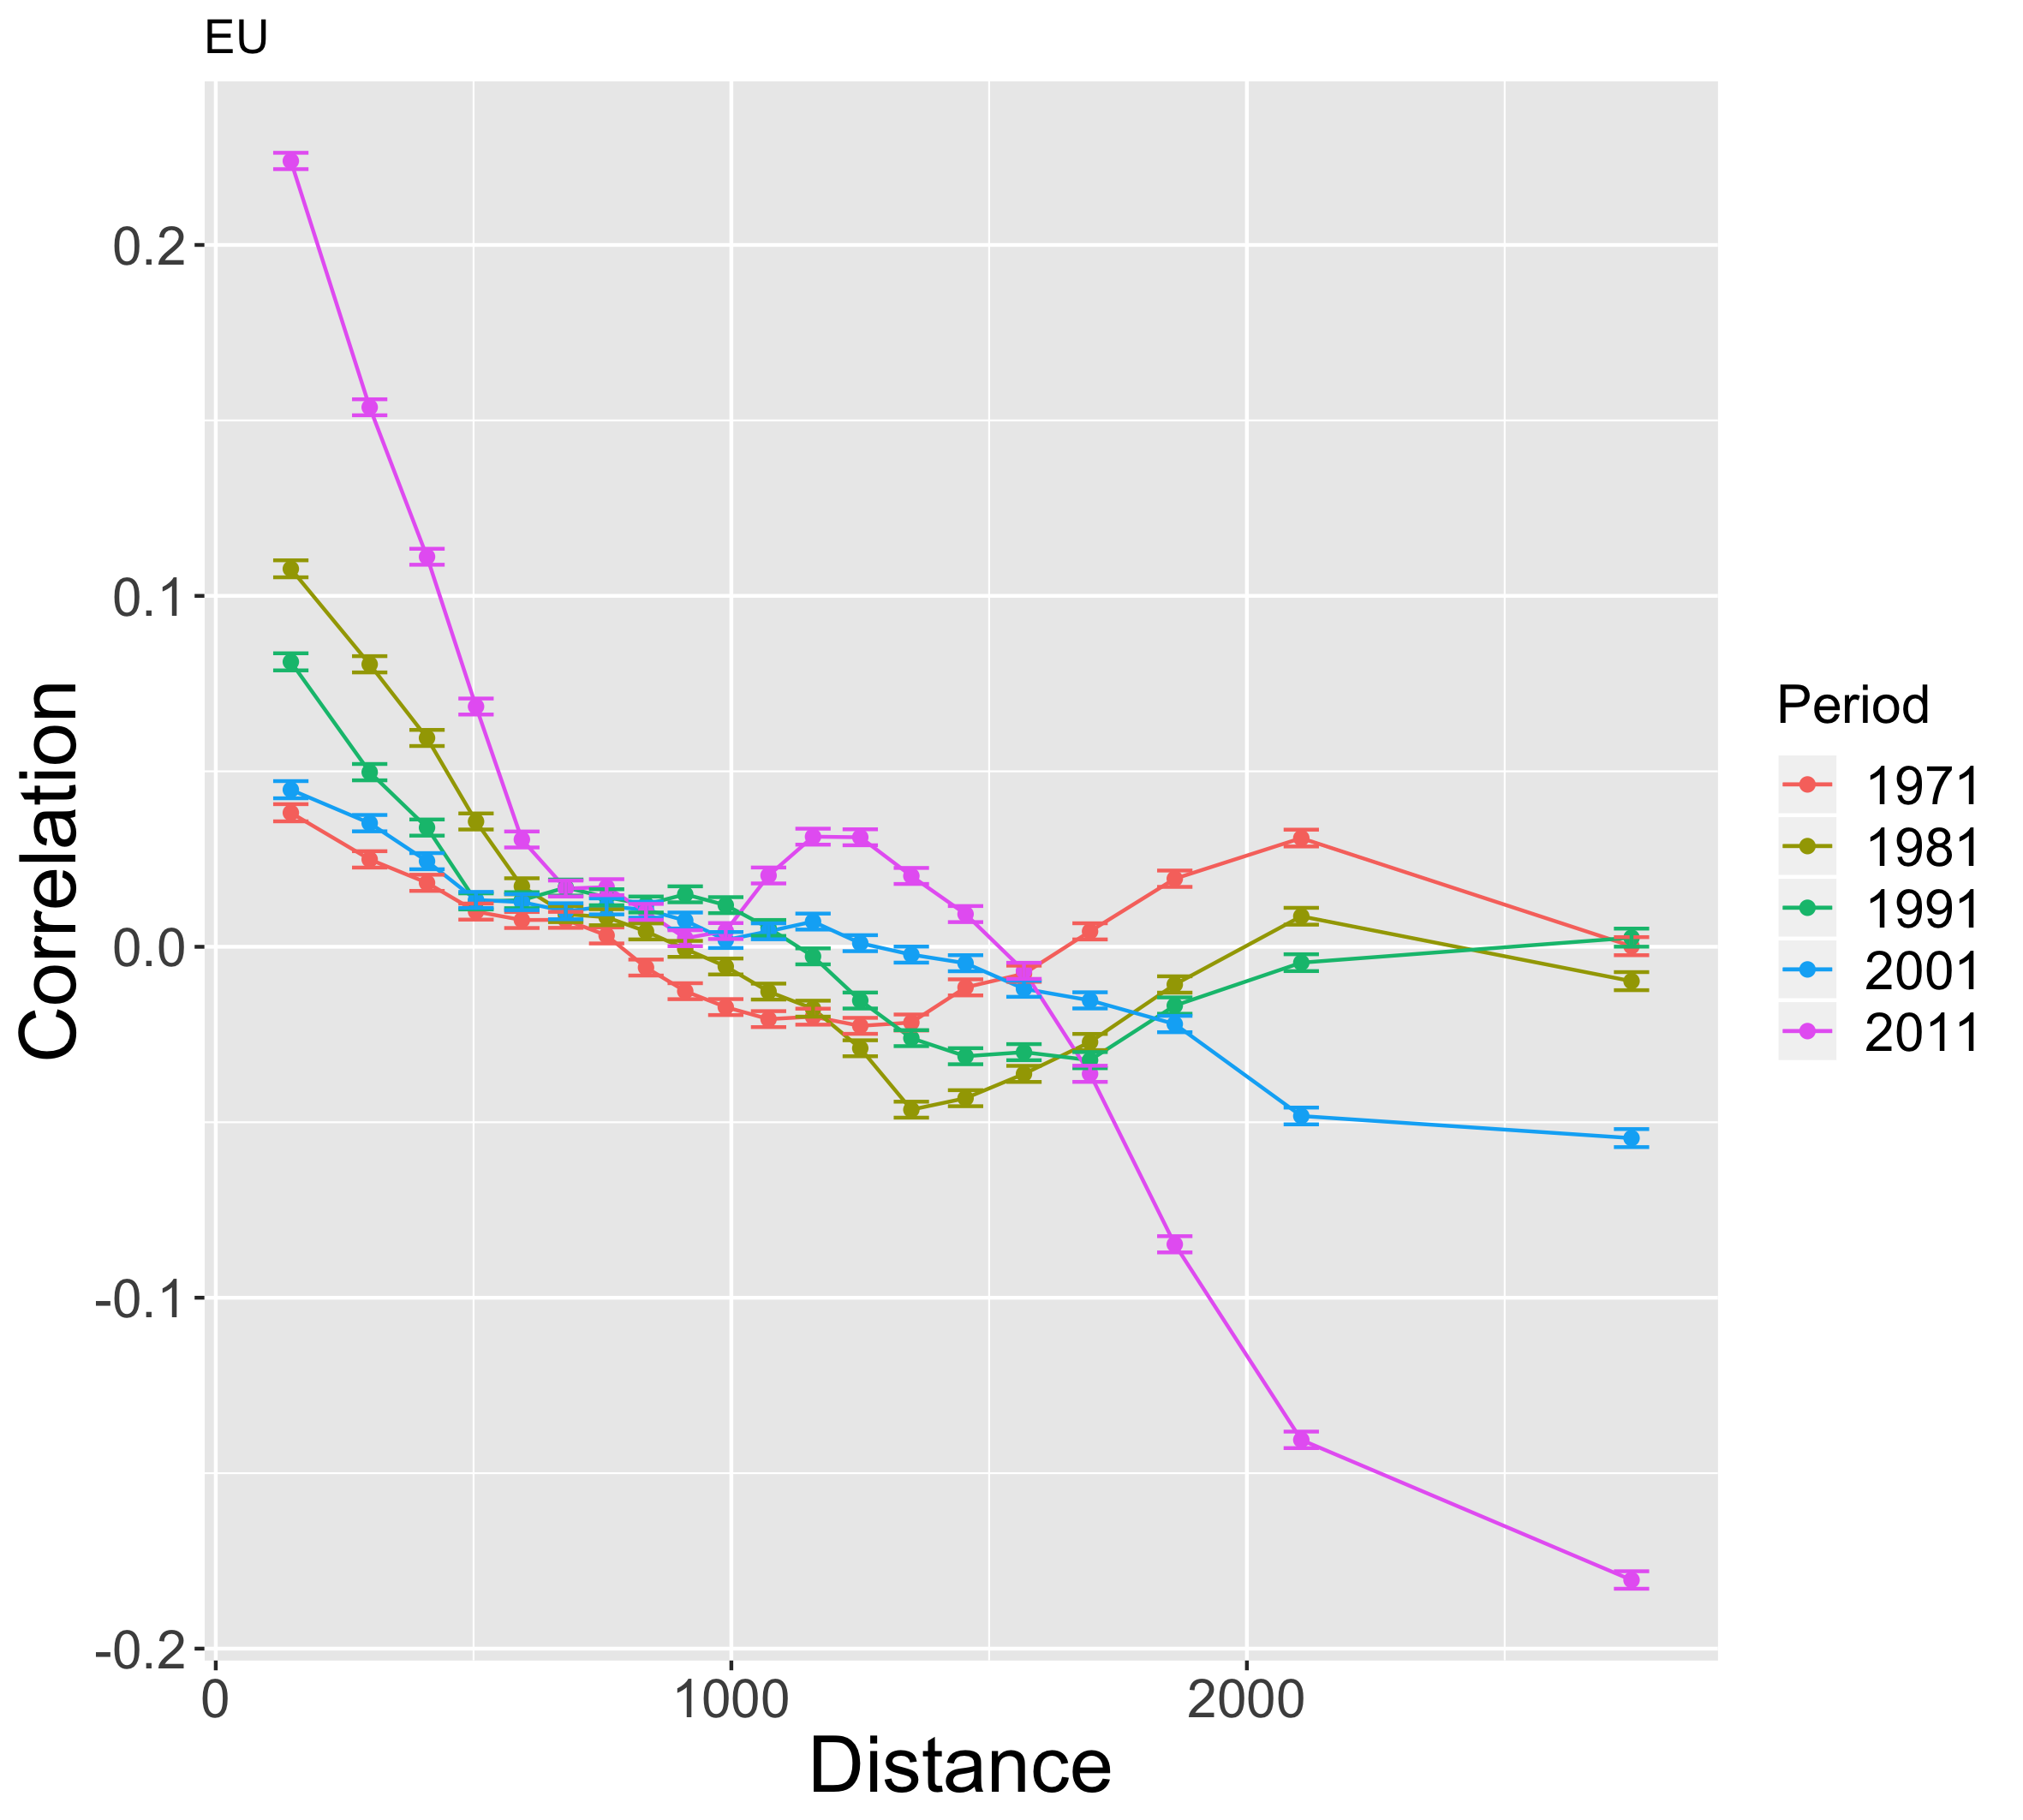
\includegraphics[width=0.49\textwidth]{figures/corrsdist_EU_quantiles21_periods5.png}

%\smallskip

%$\rightarrow$ \textit{non-linear models good candidates}


}




\sframe{Model calibration}{

% Calibrations are done for different versions of each model including more or less parameters, using distributed genetic algorithms on a computation grid through the intermediary of the OpenMOLE model exploration software [6]. 

Bi-objective calibration of 7 models for 7 city systems $\rightarrow$ use of genetic algorithms on grid, made smooth with the OpenMOLE software \url{https://next.openmole.org/}

\centering

\smallskip


\includegraphics[height=0.35\textheight]{figures/openmole.png}

\smallskip

\raggedright\justify

\footnotesize \textit{OpenMOLE: (i) embed any model as a black box; (ii) transparent access to main High Performance Computing environments; (iii) model exploration and calibration methods.}

\bigskip

\textbf{Come to the Satellite on Wednesday, and apply to the summer school !} 
\\(\texttt{https://exmodelo.org/})

}


\sframe{Comparison of models on all systems}{

%Calibration results show that: (i) at a fixed number of parameters, no model performs particularly better on all urban systems, suggesting the complementary of the innovation, economic, and network dimensions taken into account by the different models.

% global overview : Pareto plots / tabular of % effective pareto front for each system
% (requires the extraction of effective fronts)

\centering

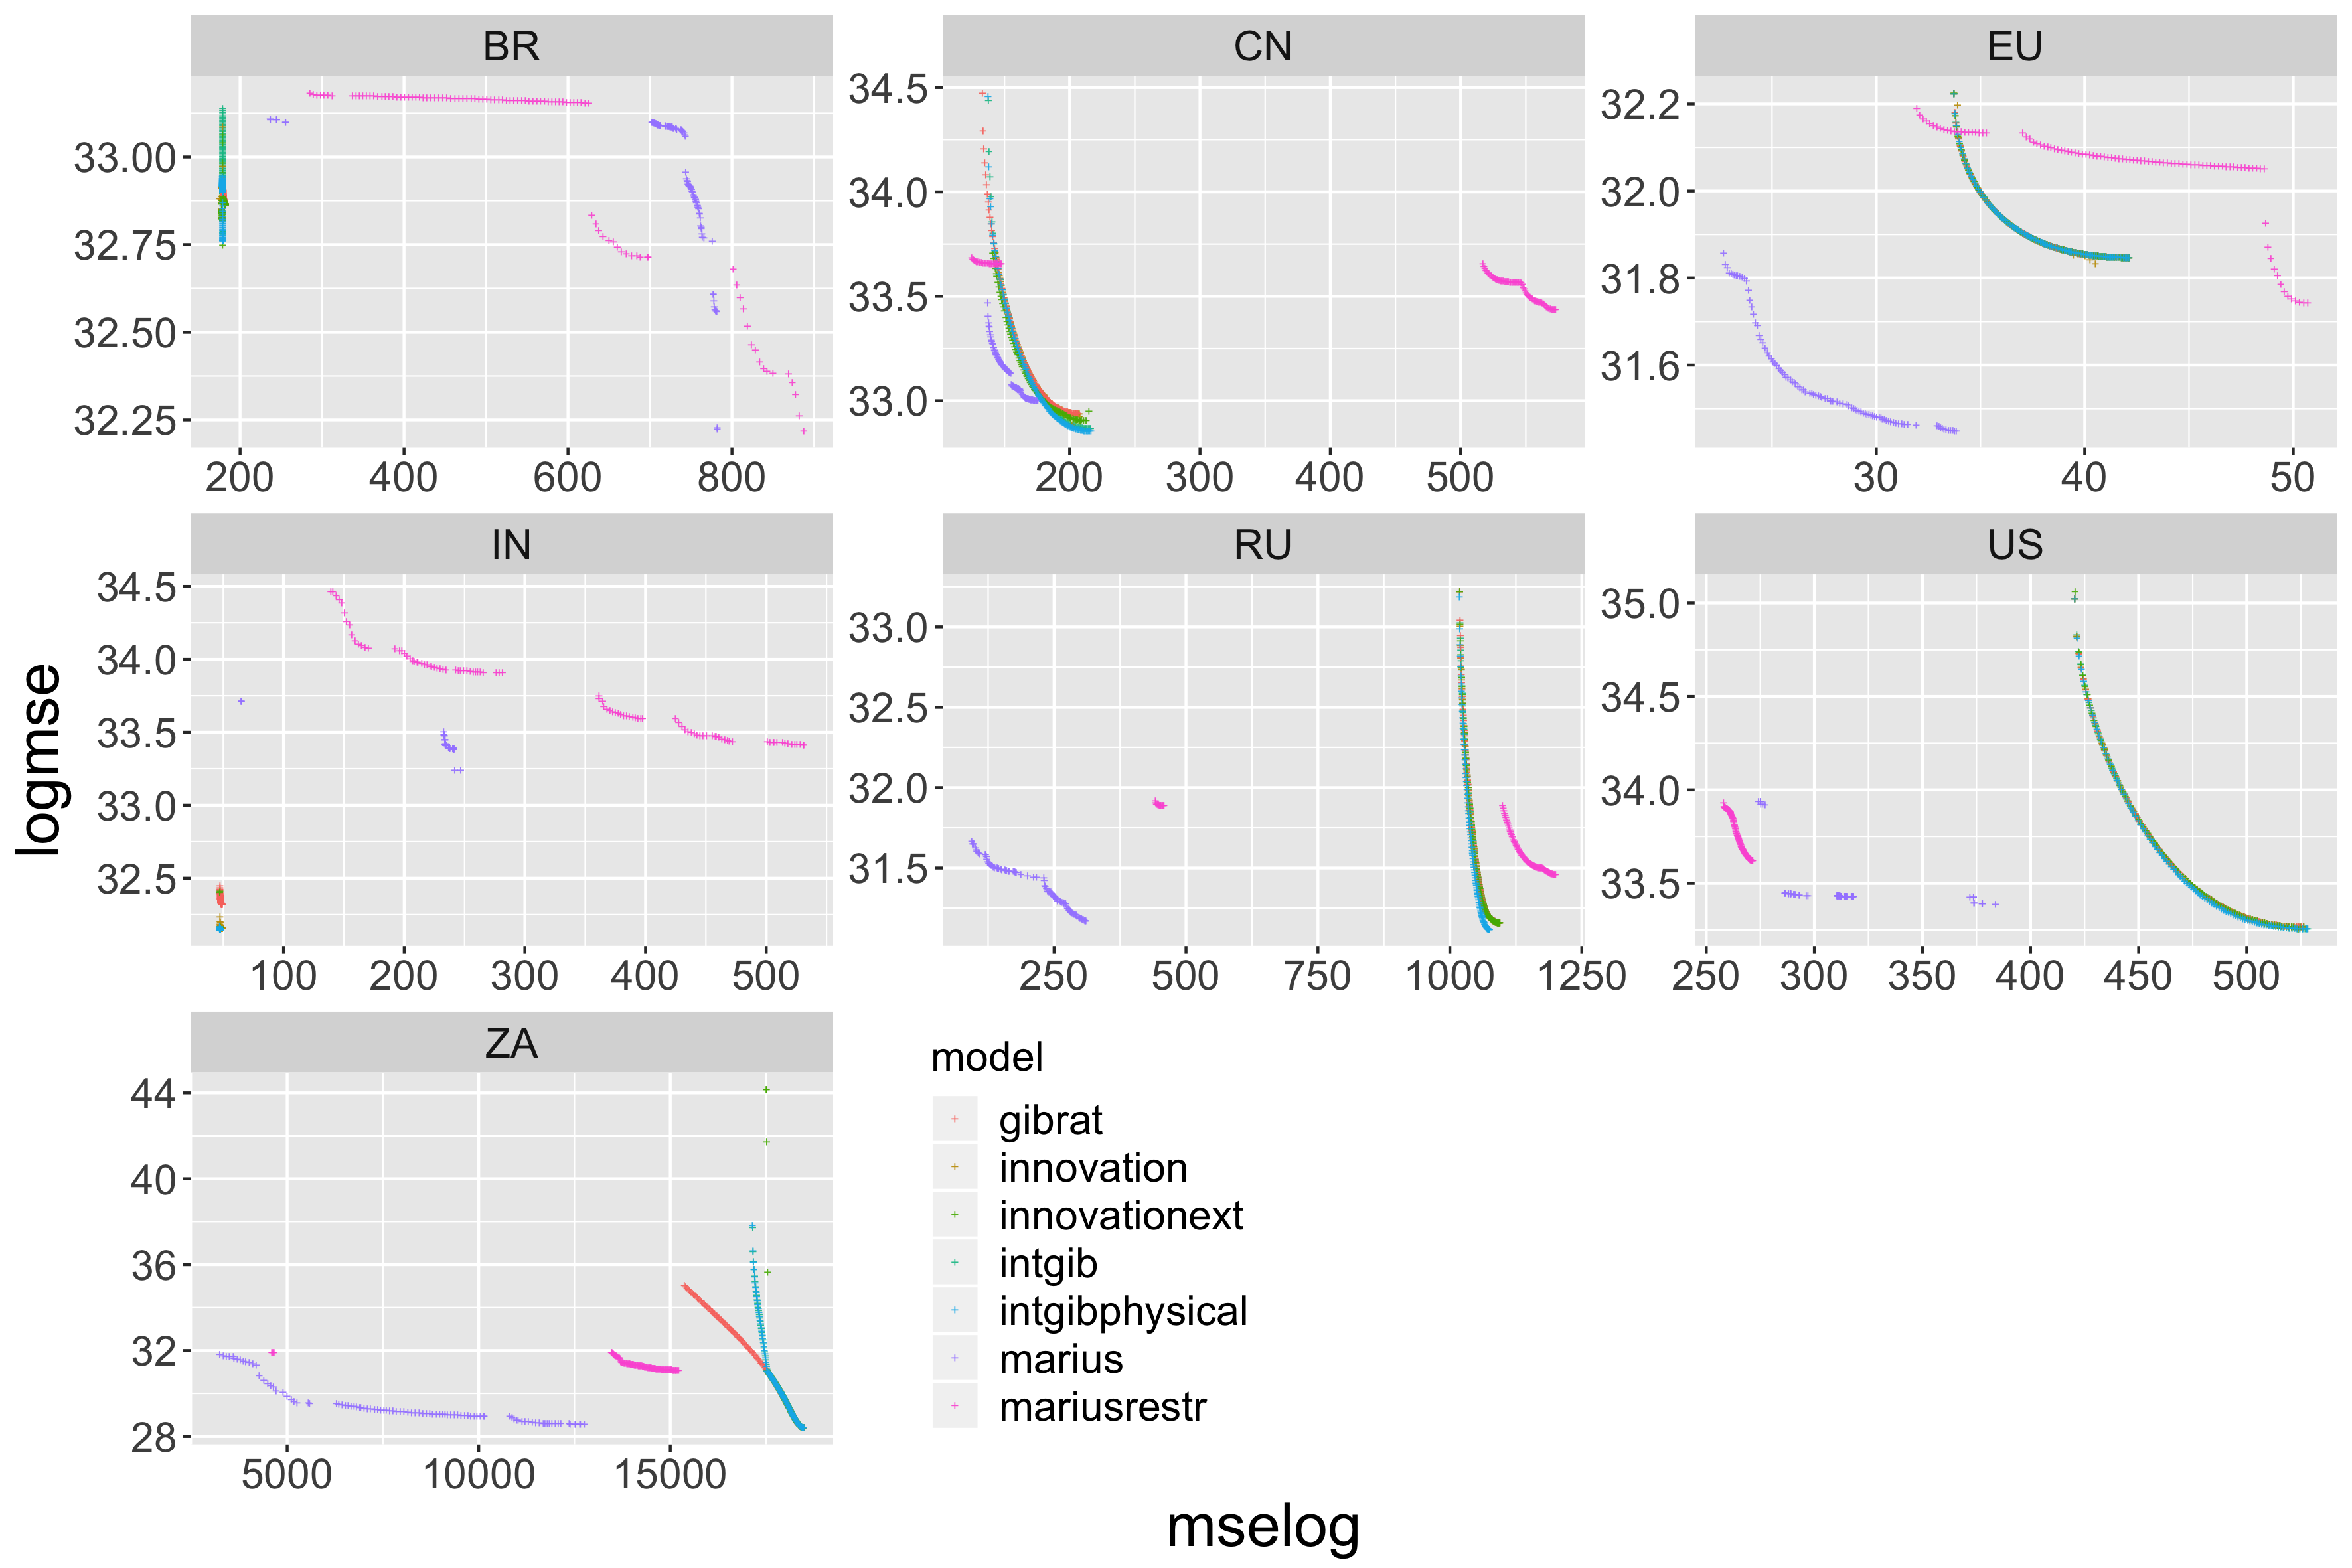
\includegraphics[width=\textwidth]{figures/allmodels_allsystems.png}

\footnotesize
\textit{Systems driven by economic exchanges: EU, US, RU, ZA}

}

\sframe{Indian urban system: direct interactions}{

% systems on which the behavior is particularly interesting ?

\centering
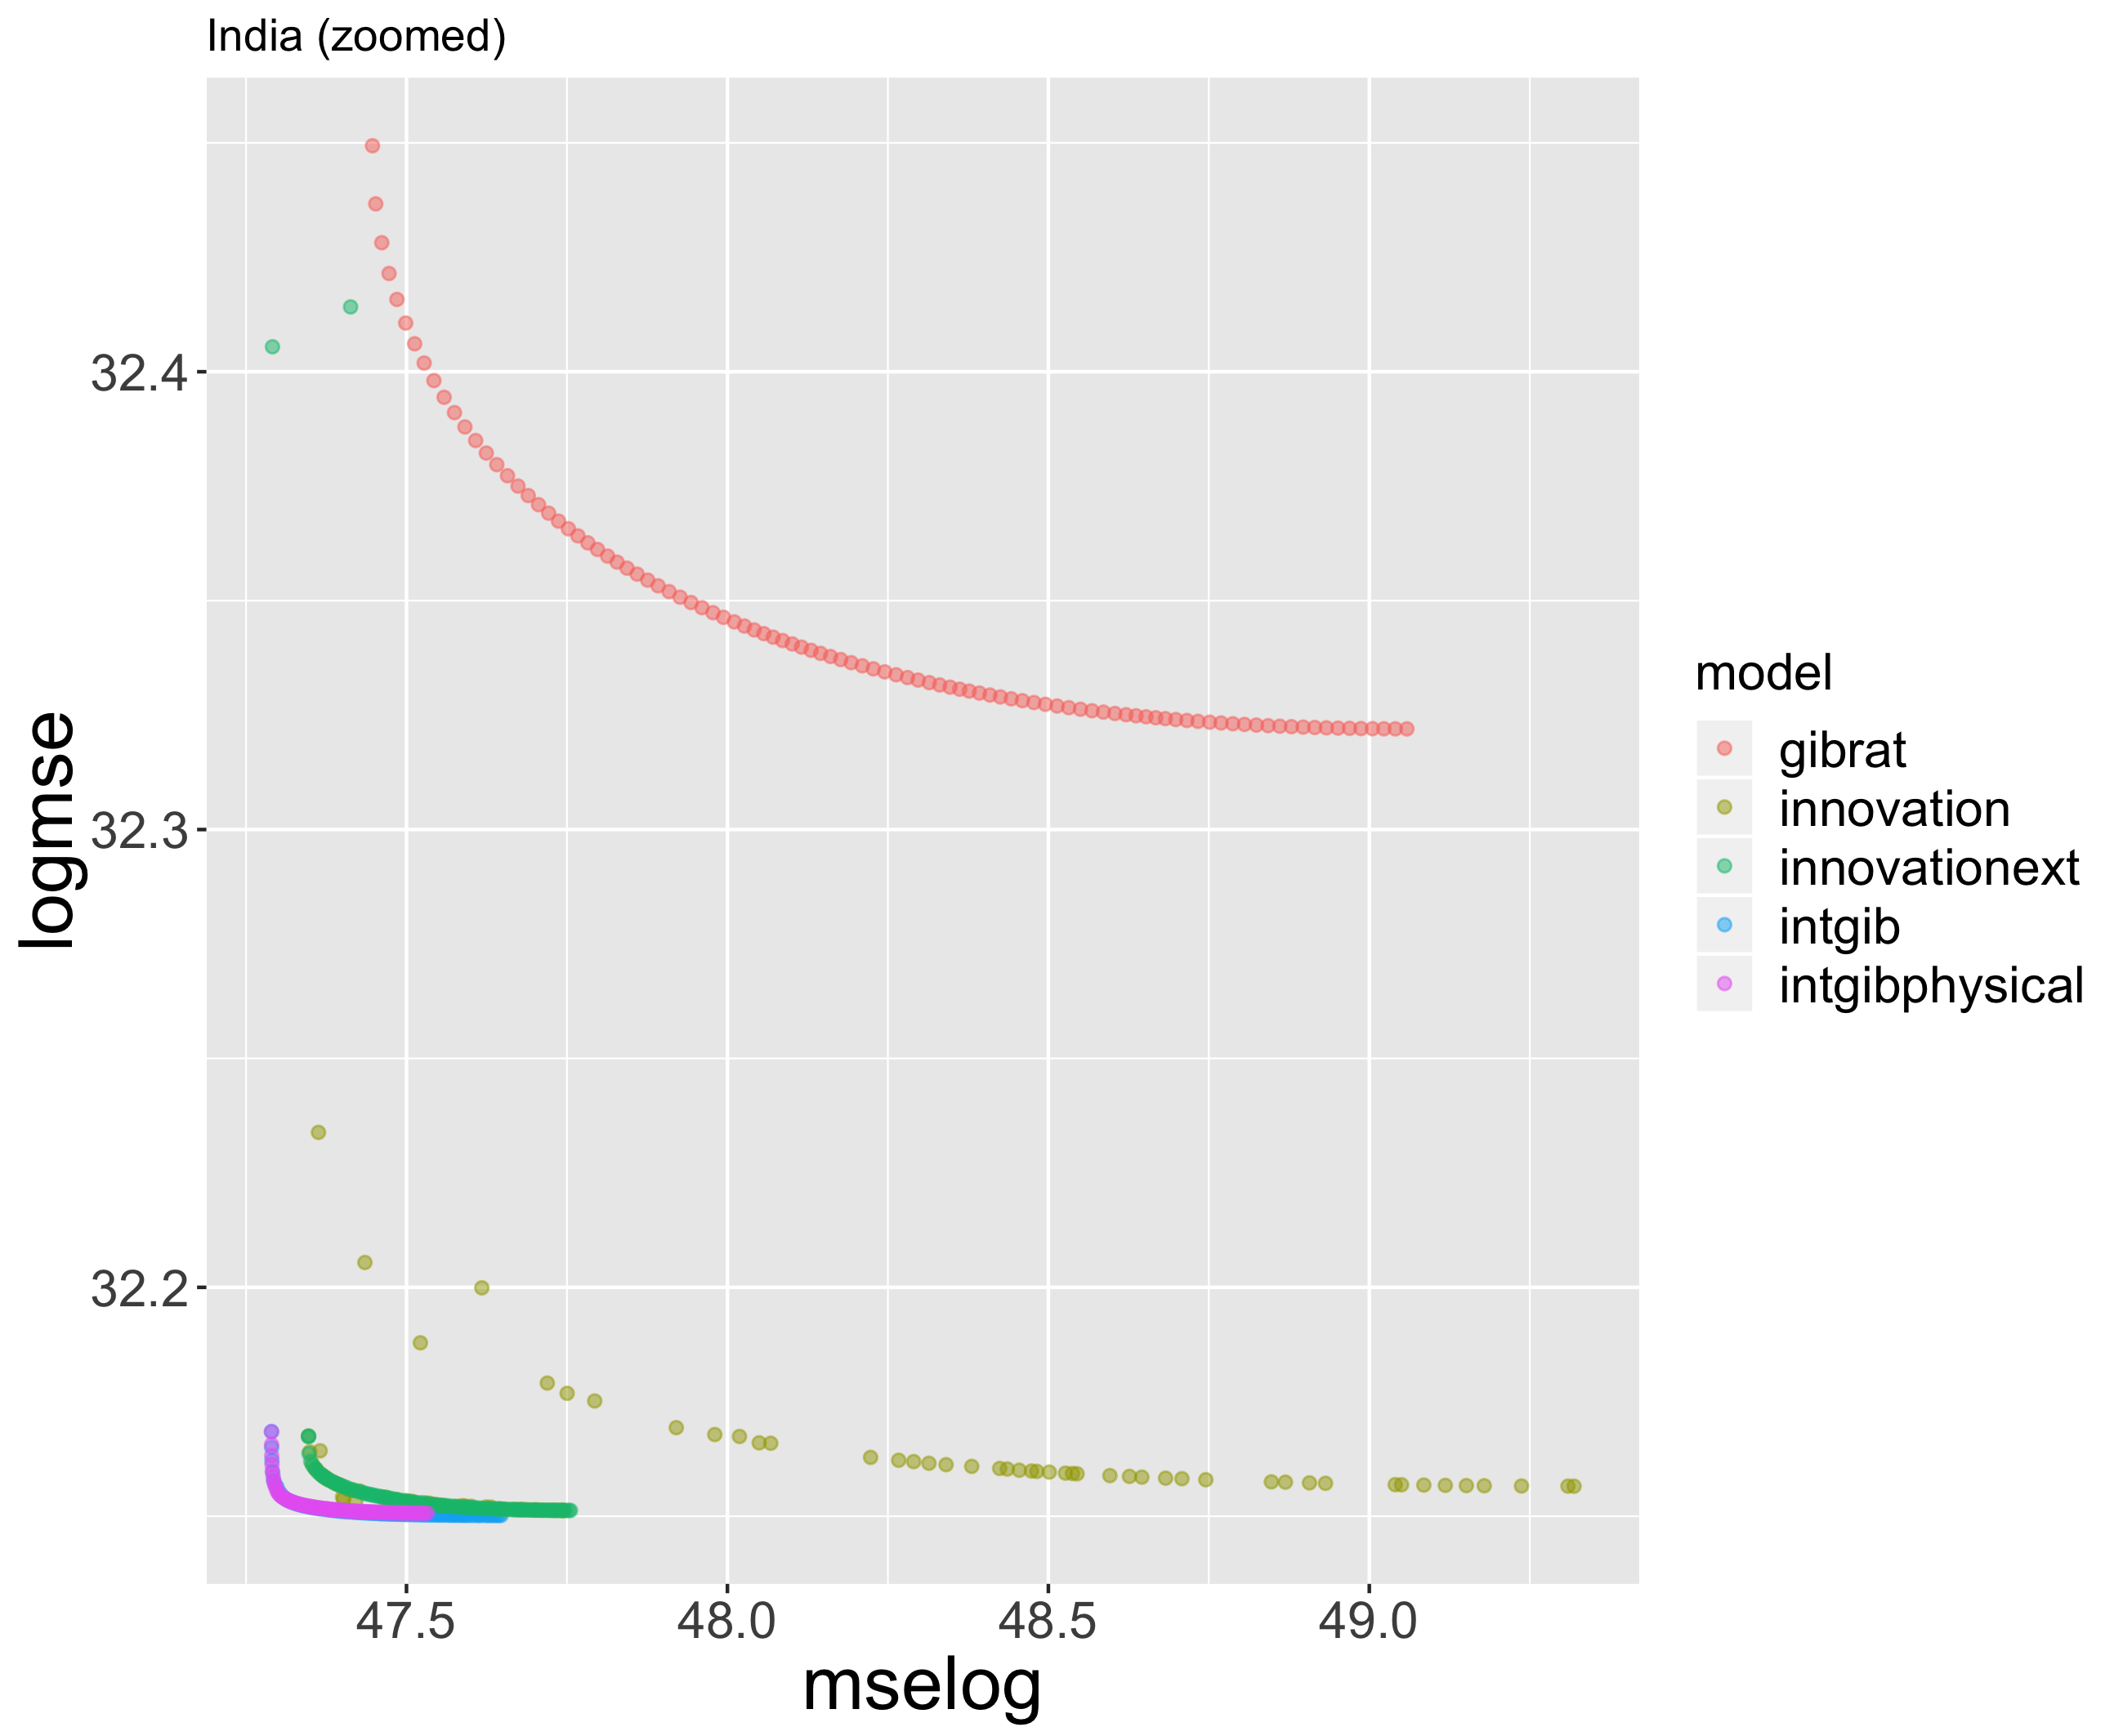
\includegraphics[width=0.9\textwidth]{figures/IN_zoomed.png}

}


\sframe{Brazilian urban system: multiple factors}{

\centering
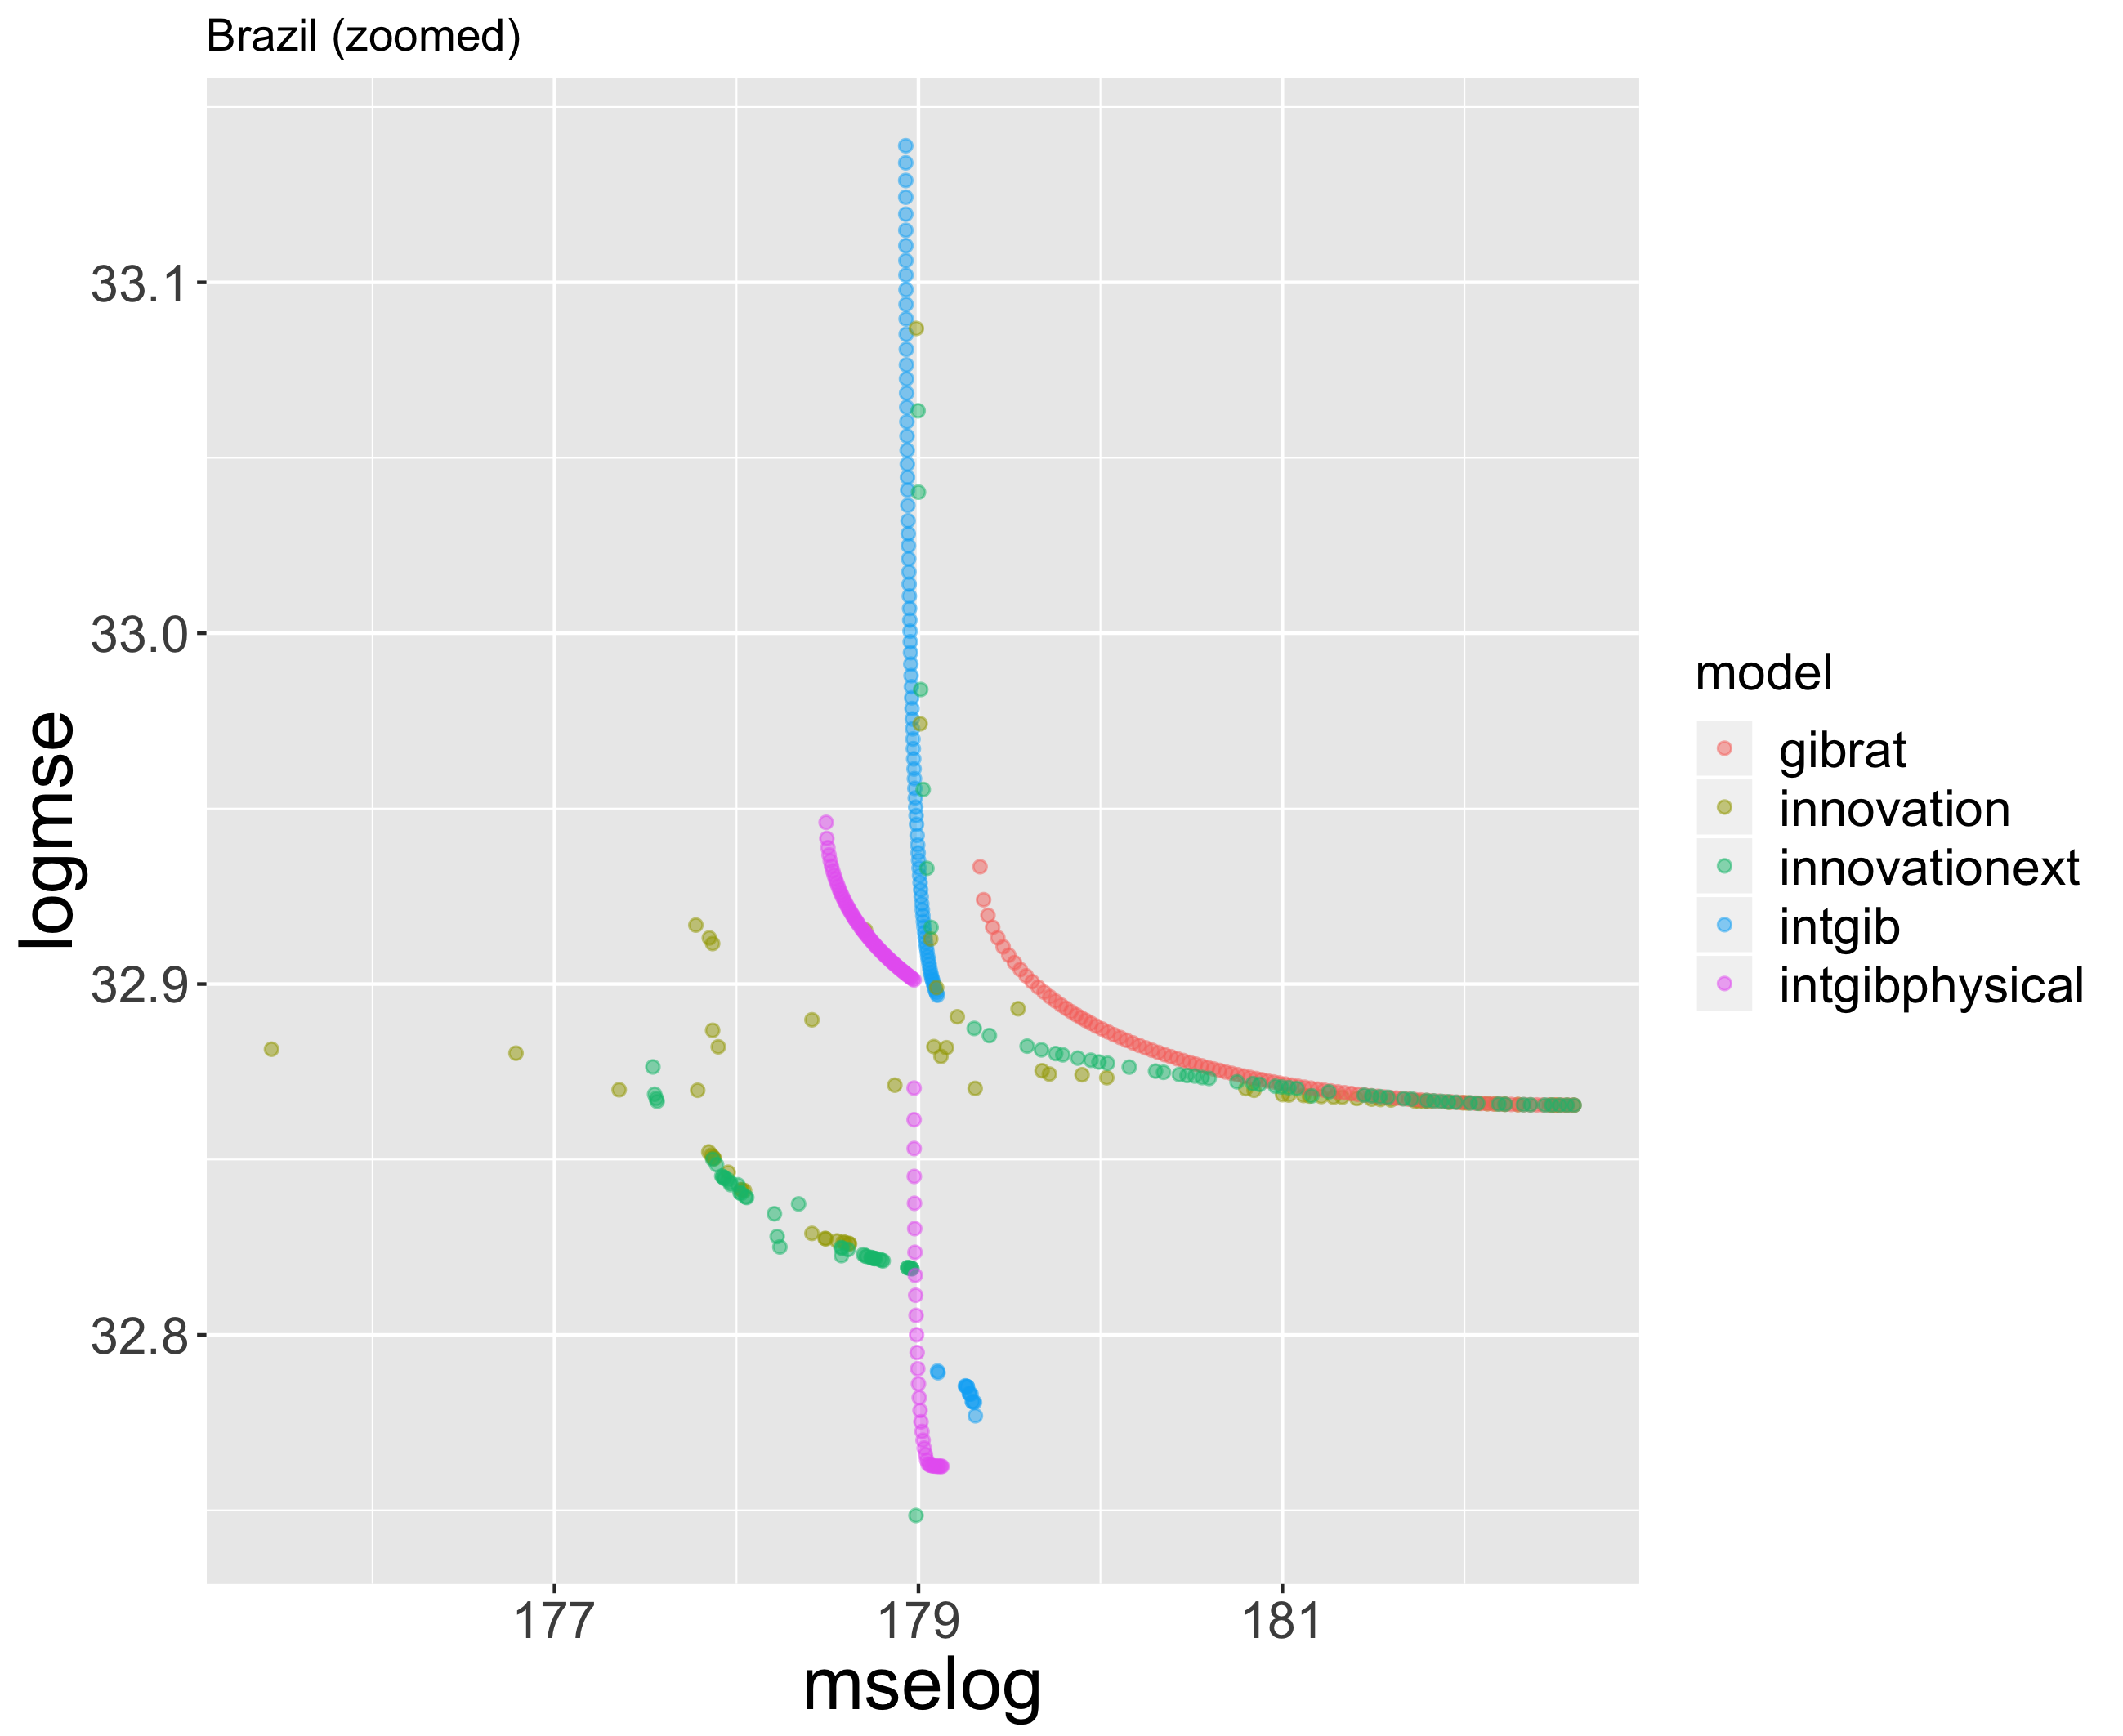
\includegraphics[width=0.9\textwidth,height=0.8\textheight]{figures/BR_zoomed.png}

\footnotesize
\textit{Importance of topography; innovation processes mostly.}

}

\sframe{China: a tight competition}{

\centering
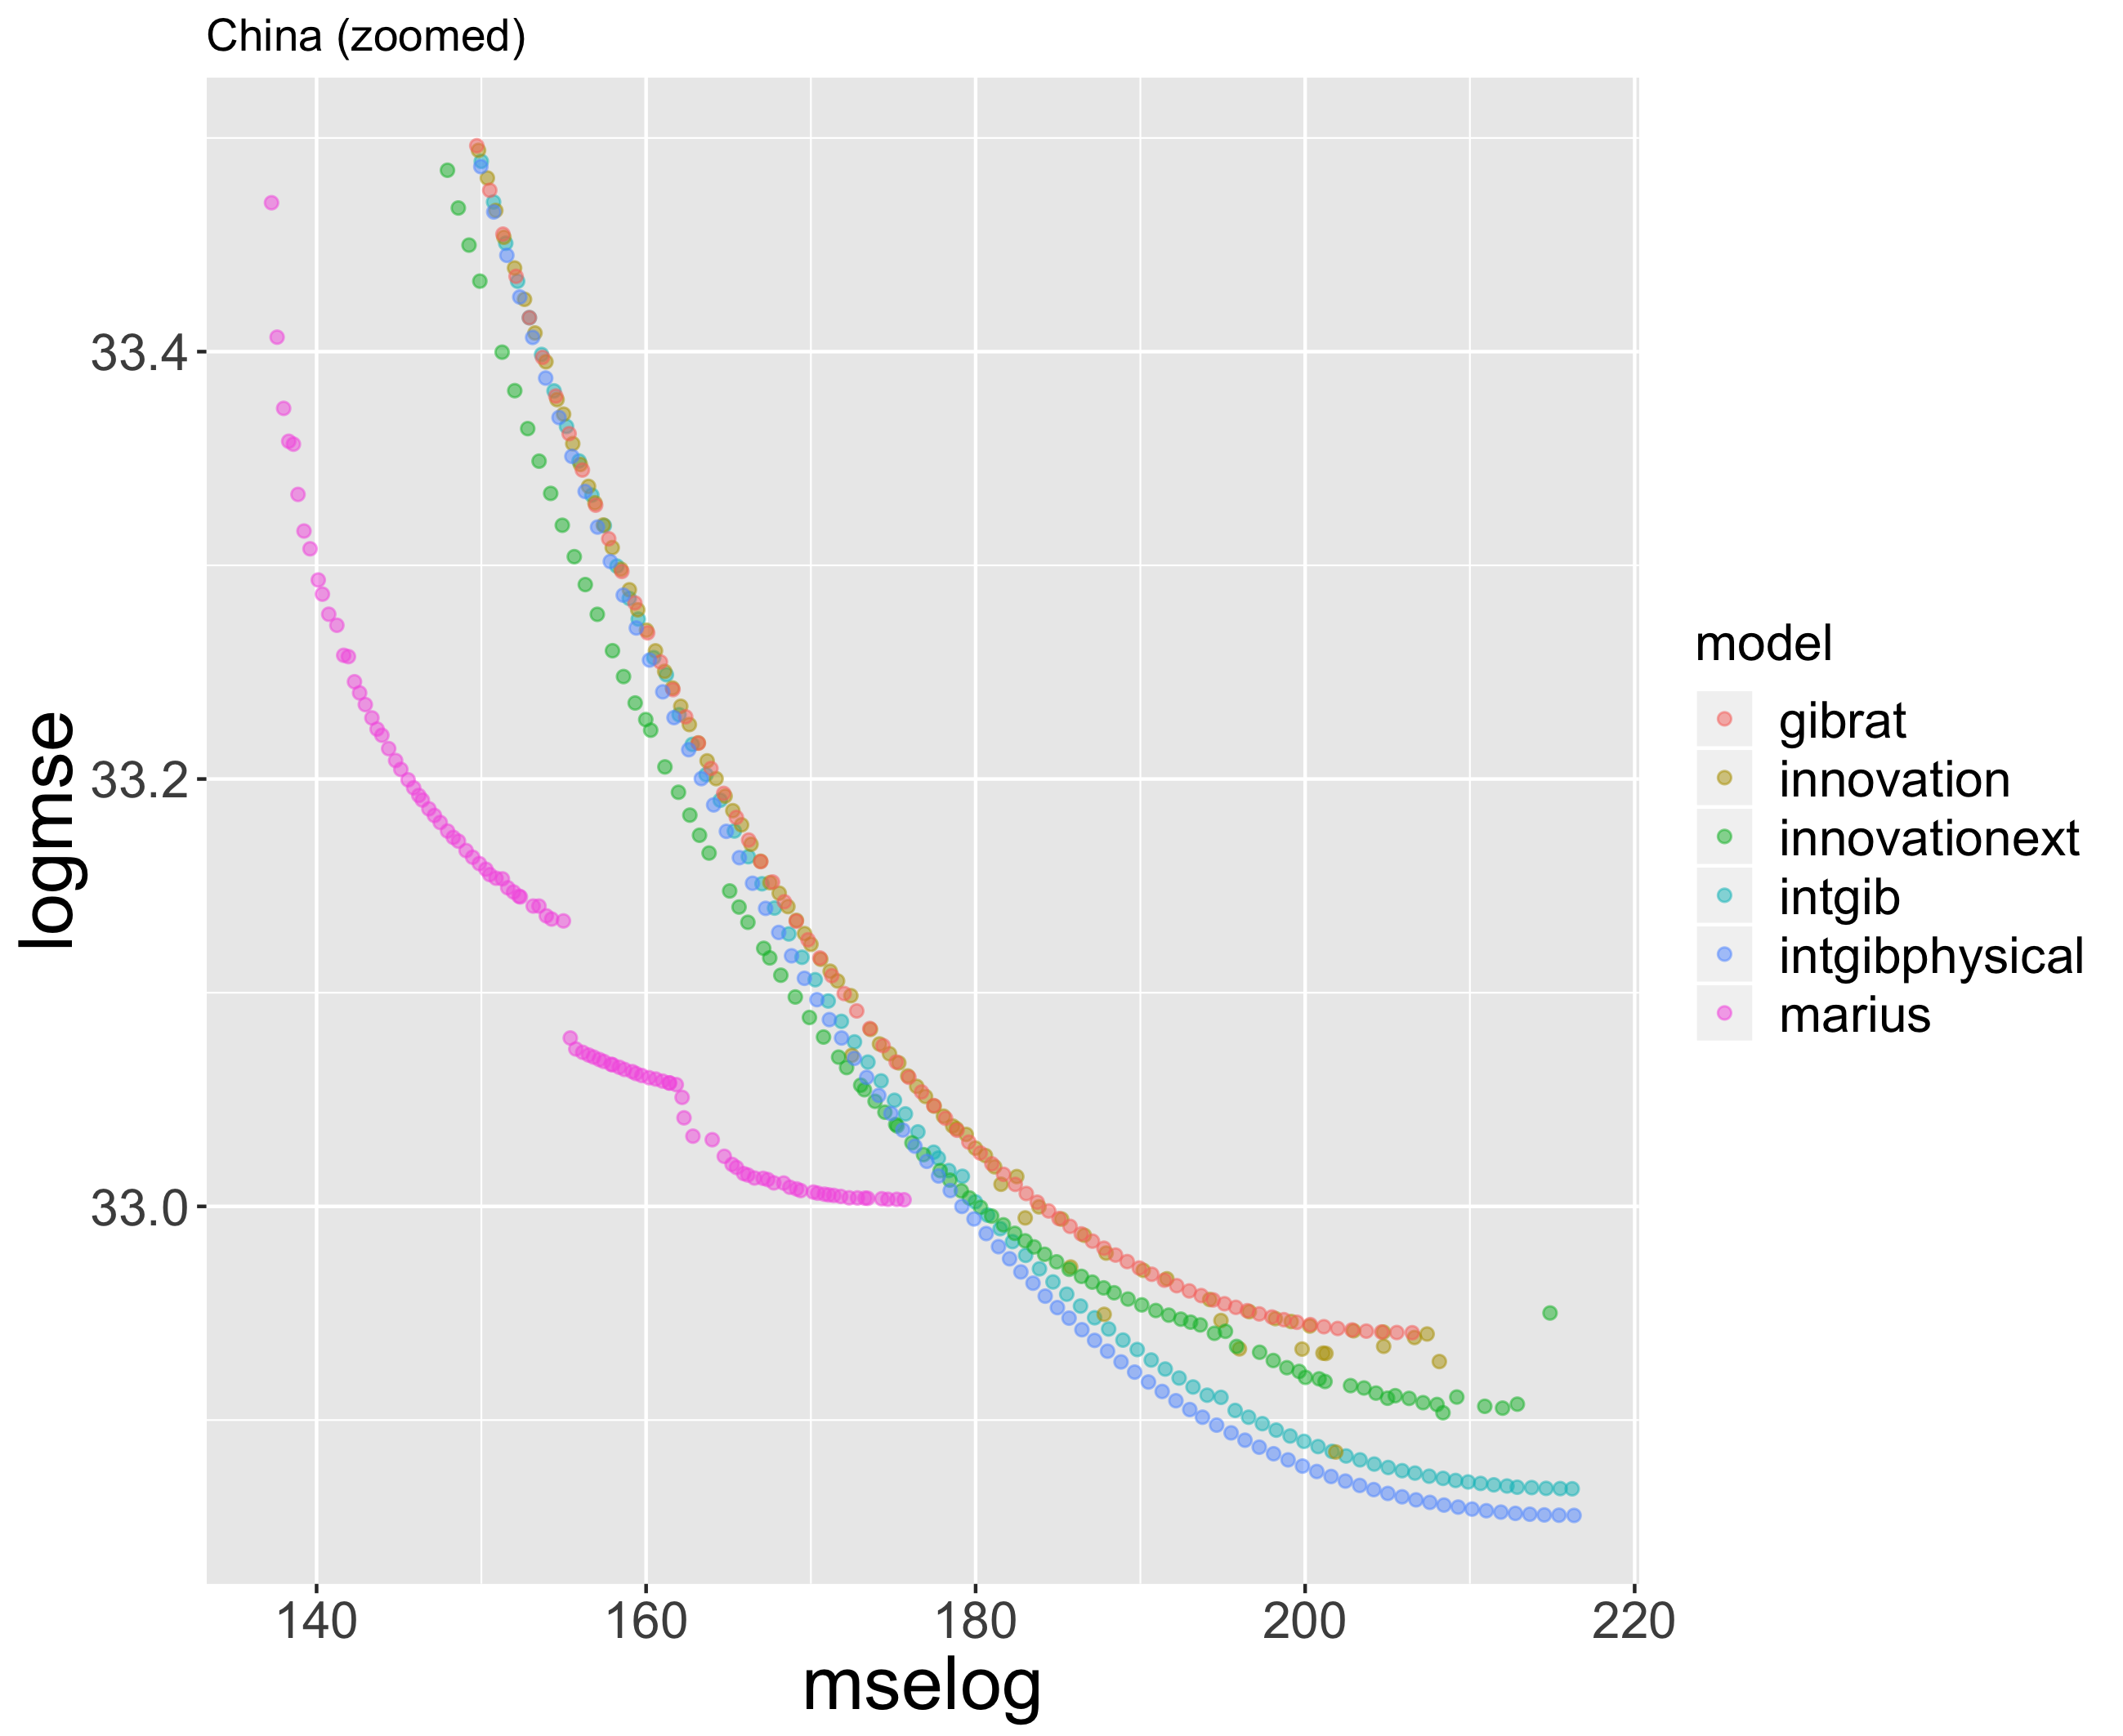
\includegraphics[width=0.9\textwidth,height=0.8\textheight]{figures/CN_zoomed.png}

\footnotesize
\textit{No clear best model: other processes in play ? (strong top-down planning)}

}



%\sframe{Results: influence of parameters}{
% add if cool results
%}

\sframe{Results: empirical AIC}{

% (ii) when adjusting for the number of parameters with an empirical information criterion [4], we find that additional components generally improve performances for all models, what reveals a high effective dimensionality of urban systems.

% - select optimal points / run empirical AIC
% OR : run on all points of the Pareto front ? -> local OK

\textit{Comparing Gibrat and Network model by correcting for the number of parameters \cite{raimbault2018indirect}: additional parameters actually improve the fit (but not always)}

\bigskip

\centering

% gib - intgib
\begin{tabular}{|c|c|c|c|c|}
\hline
System & $\Delta AIC$ (log) & $\Delta BIC$ (log) & $\Delta AIC$ (mse) & $\Delta BIC$ (mse) \\\hline
ZA & 33.82658 & 29.40496 &  -838.07184 &  -842.49347\\
CN & 20.67713 & 16.78273 & 13.40767 & 9.51327\\
BR & -263.27003 & -267.71575 & -407.55220 & -411.99792\\
IN & -85.01949 & -89.24206 & -188.16703 & -192.38960\\
RU & 50.60535 & 46.24233 & 104.94806 &  100.58503\\\hline
\end{tabular}

% marius - mariusrestr


}



\sframe{Discussion}{

% This work confirms the need for multiple complementary approaches to model urban systems and sketches a framework allowing systematic benchmarks of concurrent models for complex urban systems.


\justify

\vspace{-1cm}

\textbf{Implications}

$\rightarrow$ Complementarity of economic, innovation and direct interaction processes

\smallskip

$\rightarrow$ High dimensionality of urban systems

\bigskip



\textbf{Developments}

% future perspective : towards integrative theories / coupling of these models for multi-dimensional grasp of urban systems (more work needed to understand model coupling and role of parameters in fit improvement)
% Compare these models on synthetic city systems / with suited indicators (here relatively data-driven approach)
% - nonstat in time for some city systems ?
% - calib at the second order on correlation curves (-> new methodo approach - link with correlated synthetic data !) (many things are connected)
% saturation of models ?
% Rq : issue in calib algos (restricted vs full models : strange behavior ex the bifurcation in intgib % gibrat

$\rightarrow$ Still points on robustness to be investigated: influence of stochasticity, convergence of GA, saturation of parameters, number of cities.

\smallskip

$\rightarrow$ Towards integrated models coupling these different components ?

\smallskip

$\rightarrow$ Compare on synthetic systems of cities with appropriate indicators \cite{raimbault2018unveiling}.

\smallskip

$\rightarrow$ Calibrate at the second order (correlations), non-stationary in time.

\smallskip

$\rightarrow$ More elaborated method to compare models in a ``fair'' way (correcting for additional parameters, open question for models of simulation): model reduction ? 


}



\sframe{Conclusion}{


\justify

\vspace{-1cm}

$\rightarrow$ First step towards systematic benchmarks and multi-modeling. \textbf{Need for more systematic model exploration.} % model coupling / benchmarking

\smallskip

$\rightarrow$ Model integration and multi-scalarity ? \textbf{Need for more integrated models.}

\smallskip

$\rightarrow$ Multiple perspectives on urban systems ? \textbf{Need for more interdisciplinarity.}

\bigskip

\footnotesize

\textbf{Related works}

Raimbault, J. (2018). Indirect evidence of network effects in a system of cities. Environment and Planning B: Urban Analytics and City Science, 2399808318774335.

\url{https://halshs.archives-ouvertes.fr/halshs-01788559}

\smallskip	

Raimbault, J. (2018). Modeling the co-evolution of cities and networks. \textit{Forthcoming in Handbook of cities and networks, Rozenblat C., Niel Z., eds.} arXiv:1804.09430.

\smallskip


Raimbault, J. (2018). Caract{\'e}risation et mod{\'e}lisation de la co-{\'e}volution des r{\'e}seaux de transport et des territoires (Doctoral dissertation, Université Paris 7 Denis Diderot). \url{https://halshs.archives-ouvertes.fr/tel-01857741}




\smallskip

\textbf{Open repository} at \texttt{https://github.com/JusteRaimbault/UrbanGrowth}\\\smallskip
\textbf{Acknowledgments}: thanks to the \textit{EGI} for access to the infrastructure.


}






\sframe{Reserve slides}{

\centering

\Large

\textbf{Reserve Slides}

}

\sframe{Models settings}{

$\rightarrow$ Work under Gibrat independence assumptions, i.e. $\Covb{P_i(t)}{P_j(t)}=0$. If $\vec{P}(t+1)=\mathbf{R}\cdot \vec{P}(t)$ where $\mathbf{R}$ is also independent, then $\Eb{\vec{P}(t+1)}=\Eb{\mathbf{R}}\cdot\Eb{\vec{P}}(t)$. Consider expectancies only (higher moments computable similarly)

\medskip

$\rightarrow$ With $\vec{\mu}(t)=\Eb{\vec{P}(t)}$, we generalize this approach by taking $\vec{\mu}(t+1)=f(\vec{\mu}(t))$

}



\sframe{Network model}{

Direct network interaction model \cite{raimbault2018indirect}:

\medskip

Let $\vec{\mu}(t)=\Eb{\vec{P}(t)}$ cities population and $(d_{ij})$ distance matrix

\medskip

Model specified by

\[
f(\vec{\mu}) = r_0\cdot \mathbf{Id}\cdot \vec{\mu} + \mathbf{G}\cdot \mathbf{1} + \mathbf{N}
\]

 with 
\begin{itemize}
\item $G_{ij} = w_G\cdot \frac{V_{ij}}{<V_{ij}>}$ and $V_{ij} = \left(\frac{\mu_i\mu_j}{\sum{\mu_k}^2}\right)^{\gamma_G} \exp{(-d_{ij}/d_G)}$
\item $N_{i} = w_N \cdot \sum_{kl} \left(\frac{\mu_k\mu_l}{\sum\mu}\right)^{\gamma_N}\exp{(-d_{kl,i})/d_N}$ where $d_{kl,i}$ is distance to shortest path between $k,l$ computed with slope impedance ($Z=\left(1+\alpha/\alpha_0\right)^{n_0}$ with $\alpha_0\simeq 3$)
\end{itemize}


}


\sframe{Innovation diffusion}{

Favaro-Pumain model \cite{favaro2011gibrat}:

\medskip

1) Diffuse innovations according to 
\[
\delta_{c,i,t} = \frac{\sum_j p_{c,j,t-1}^{s_c} \exp{(-\lambda_s d_{ij})}}{\sum_c \sum_j p_{c,j,t-1}^{s_c} \exp{(-\lambda_s d_{ij})}}
\]

\medskip

2) Update population with $G_{ij}$ (see network model) such that
\[
V_{ij}= \frac{p_i p_j}{(\sum_k p_k)^2} \exp{(-\lambda_m d_{ij} \prod_c \delta_{c,i}^{\phi_c})}
\]
with $\phi_c = \sum_i p_{i,c}/\sum_{i,c} p_{i,c}$

\medskip

3) Introduce innovation with utility $s_{c+1} = g_0 \cdot s_c$ in a randomly chosen city with a hierarchy parameter $\alpha_I$, if global adoption share $\phi_c$ is larger than a threshold $\theta_I$. Initial utility $s_0$ is a parameter. New innovation has an initial penetration rate $r_I$ in the city.

}

\sframe{Economic exchanges}{

Marius model \cite{10.1371/journal.pone.0138212}:

\medskip

Initial wealth as a power law of population (exponent $\alpha_W$)

\medskip

1) Update supply and demands as superlinear functions of population (exponents $\alpha_S,\alpha_D$)

\medskip

2) Exchange goods according to a gravity potential of interaction (distance decay $d_M$), supplies and demands; update wealth accordingly

\medskip

3) Update population such that population difference is a power law of wealth difference (economic multiplier $e_M$ and exponent $\alpha_P$)

}


\sframe{Benchmarked models}{

\begin{enumerate}
	\item Gibrat model: 1 param. $r_0$
	\item Direct interaction model (geographical distance): 4 param. $r_0,w_G,\gamma_G,d_G$
	\item Physical network interaction model (topographical distance: 4 param. $r_0,w_G,\gamma_G,d_G$
	\item Innovation diffusion model (simplified): 4 param. $r_0,w_I,\lambda_s,\lambda_m$ (other parameters at default values from \cite{favaro2011gibrat})
	\item Innovation diffusion model (full): 9 param. $r_0,w_I,\lambda_s,\lambda_m,s_0,g_0,r_I,\alpha_I,\theta_I$
	\item Restricted Marius model: 4 param. $e_M,\alpha_S,\alpha_D,d_M$
	\item Marius model: 6 param. $e_M,\alpha_S,\alpha_D,d_M,\alpha_W,\alpha_P$
\end{enumerate}

}



\sframe{Model calibration}{

% number of runs (equivalent / year) ; caracs of NSGA2 ; convergence for each model/system

Genetic algorithm NSGA2:

\bigskip

\begin{itemize}
	\item Around 40000 generations (4e6 model runs)
	\item Population $\mu = 100$
	\item Convergence tested with hypervolume relative variation
\end{itemize}


}


%%%%%%%%%%%%%%%%%%%%%
\begin{frame}[allowframebreaks]
\frametitle{References}
\bibliographystyle{apalike}
\bibliography{/Users/juste/ComplexSystems/CityNetwork/Biblio/Bibtex/CityNetwork,biblio}
\end{frame}
%%%%%%%%%%%%%%%%%%%%%%%%%%%%




\end{document}









